\documentclass{article}
\usepackage{fullpage}
\usepackage{indentfirst}
\usepackage{amsmath}
\usepackage{amsfonts}
\usepackage{MnSymbol}
\usepackage{array}
\usepackage{tipa}
\usepackage{tikz}
\usepackage{tikz-qtree}
\usetikzlibrary{matrix, arrows, automata}
\usepackage{gb4e}
\noautomath
\usepackage{verbatim}
\newcommand{\Y}{$\checkmark$}
\newcommand{\N}{\ding{55}}
\newcommand{\R}{$\Rightarrow$}
\newcommand\myeq{\mathrel{\stackrel{\makebox[0pt]{\mbox{\normalfont\tiny def}}}{=}}}
\newcommand\se{\small+}
\newcommand{\ap}{\approx}
\newcommand{\all}{\forall}
\title{The Computational Properties of Tonal Geometry: Yip(1989) and Bao(1990)}
\author{Chris Oakden}
\begin{document}
\maketitle
\section{Tonal Geometry in Yip (1989) and Bao (1990)}
This section introduces the tonal geometries proposed in Yip (1989) and Bao (1990), beginning with an informal description of the representations. A concrete example from the Zhenhai dialect (Rose 1990, Chen 2000) is presented using each representation (this dialect is the focal point of comparison between the two dialects in subsequent sections). We then examine the basic properties of these geometries by constructing model of the Zhenhai tonal structures. In doing so, we show that these representations can be defined explicitly in model theory. We also offer a general description of Yip and Bao models which generalizes over any structure in the respective geometries, and includes explicit definitions and axioms which govern the structure. General examples are given to explicate the definitions of the models. 
\subsection{Yip (1989)}
Yip (1989) draws on earlier work on the branching structure of affricates (Clements 1985, Sagey 1986) to propose a novel model of tonal geometry. This model is inspired by characteristics of contour tones which have parallels in the segmental domain, namely association of contour tones as units as well as edge effects. Yip proposes a geometry in which `tonal features hang off a root node', much like Sagey's (1986) branching structure for affricates. The root node associates to a TBU (which Yip argues to be the syllable in Chinese languages) mirroring the association between a consonantal root node and a `C' segment in Sagey's terms. The tonal root itself is a register node specified by the binary feature [$\pm$upper] which bisects the vocal register. This node dominates up to two terminal tonal nodes, specified as [$\pm$raised] (borrowing Pulleyblank's (1986) terminology), further dividing up the vocal space. Contour tones are thus sequences of [+raised][-raised] or [-raised][+raised]. Note that the upper bound on root node branching is two; Yip argues that ultra-complex tonal structures (convex and concave) are the result of multiple root nodes. Compare Sagey's model of an affricate to Yip's model of a contour tone below.
\begin{center}
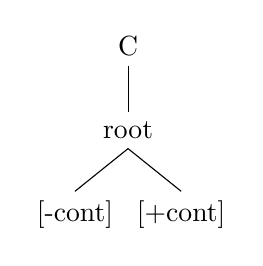
\begin{tikzpicture}[baseline=(current bounding box.north)]
\Tree [.C [.root [.{$[$-cont$]$} ] [.{$[$+cont$]$} ]]];
\end{tikzpicture}
\hspace{1cm}
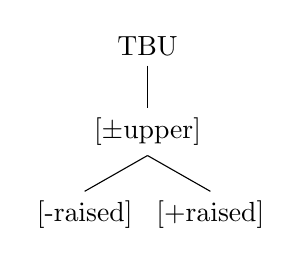
\begin{tikzpicture}[baseline=(current bounding box.north)]
\Tree [.TBU [.{$[\pm$upper$]$} [.{$[$-raised$]$} ] [.{$[$+raised$]$} ]]];
\end{tikzpicture}
\end{center}
Our goal is to offer an explicit definition of this structure in model theoretic terms. To do so, several questions must be addressed: what are the constituent parts of such a model, how do they relate to the elements of Yip's tonal geometry, how do they relate \emph{to one another}, and how do we define these relations? We can represent these structures by defining models over them. These models consists of a domain of elements which correspond to the nodes (TBU, register, terminal root node) in Yip's model. Domain elements are labeled---as either a TBU node, register node, or tonal node---via a set of \emph{unary relations} which specify a particular feature. Domain elements relate to one another via a set of \emph{binary functions}; these functions correspond to relations between nodes in Yip's model, such as tone-to-TBU association, as well as dominance (within the internal structure of the tone). Additionally, a binary function will impose a linear order on polysyllabic forms, as well as sequences of tonal terminal nodes in contour tones. We thus define the signature $\zeta_{y}$ for a model of Yip's tonal geometry. Note that the feature [$\pm$upper] is designated by [$\pm $u], and that [$\pm$raised] is represented by the conventional `h' and `l' respectively:
\begin{equation}
\zeta_{y} \myeq \{P_{\sigma}, P_{+u}, P_{-u}, P_{h}, P_{l}; \alpha, \delta, succ\}
\end{equation} 
This signature comprises five unary relations; these label domain elements as syllable nodes, register nodes ($P_{+u}$, $P_{-u}$), or terminal tonal nodes ($P_{h}$, $P_{l}$). The three binary functions include a function which defines association from TBUs to tonal root nodes ($\alpha$), a dominance function for the internal structure of tones ($\delta$), and a successor relation which imposes a linear order on elements in the model ($succ$). \par
We illustrate with an example. In Yip's tonal geometry, the Zhenhai word \textipa{f\~a}$^{11}$ \textipa{k\;E}$^{334}$ [L.MH] `bedroom' can be represented as follows: the first syllable associates to a [-upper] register node, which then dominates a [-raised] terminal node; the second syllable associates to a [+raised] register node which dominates two terminal nodes which are specified as [-raised] and [+raised] (creating a rising contour).
\begin{center}
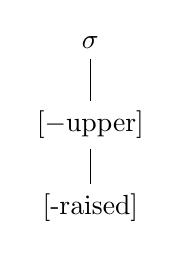
\begin{tikzpicture}[baseline=(current bounding box.north)]
\Tree [.$\sigma$ [.{$[-$upper$]$} [.{$[$-raised$]$} ] ]];
\end{tikzpicture}
\hspace{1em}
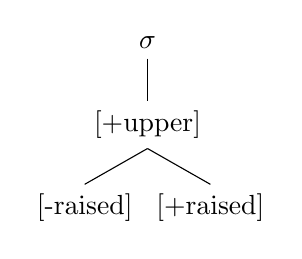
\begin{tikzpicture} [baseline=(current bounding box.north)]
\Tree [.$\sigma$ [.{$[+$upper$]$} [.{$[$-raised$]$} ] [.{$[$+raised$]$} ]]];
\end{tikzpicture}
\end{center}
We define a model $\mathcal{M}^{Y}_{zh}$ for this structure over a domain of elements, and with a series of unary relations and binary functions as below. 
\begin{equation}
\begin{aligned}
\mathcal{M}^{Y}_{zh} \myeq \langle \mathcal{D}; P_{\sigma}, P_{+u}, P_{-u}, &P_{h}, P_{l}; \alpha(x)\ap y, \delta(x)\ap y, succ(x)\ap y \rangle \\
\mathcal{D} &= \{1, 2, 3, 4, 5, 6, 7\} \\
P_{\sigma} &= \{1, 2\} \\
P_{+u} &= \{4\} \\
P_{-u} &= \{3\} \\
P_{h} &= \{7\} \\
P_{l} &= \{6\} \\
\alpha(x)\ap y &= \begin{cases} 3 & x=1 \\ 4 & x=2 \end{cases} \\
\delta(x)\ap y &= \begin{cases} 3 & x=5 \\ 4 & x\in \{6,7\} \end{cases} \\
succ(x)\ap y &= \begin{cases} 2 & x\in \{1,2\} \\ 4 & x\in \{3,4\} \\ 6 & x=5 \\ 7 & x\in\{6,7\} \end{cases} \\
\end{aligned}
\end{equation}
Graphically, the model $\mathcal{M}^{Y}_{zh}$ is:
\begin{center}
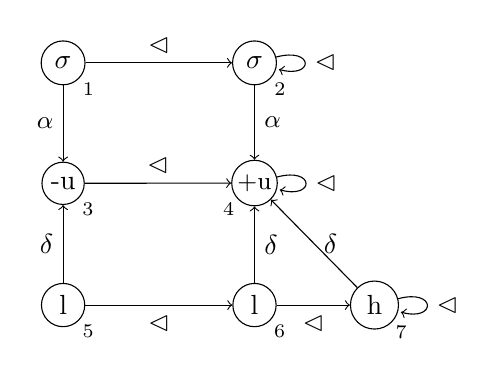
\begin{tikzpicture} [baseline = (x.base)]
\matrix (m) [matrix of nodes, column sep = 2em, row sep = 2em]{
\node[draw,circle, inner sep =3pt, label ={[label distance = -3pt] below right:\scriptsize1}](x){$\sigma$}; & &  \node[draw,circle, inner sep =3pt, label ={[label distance = -3pt] below right:\scriptsize2}](x2){$\sigma$};\\
\node[draw,circle, inner sep =2pt, label ={[label distance = -3pt] below right:\scriptsize3}](y){-u}; & & \node[draw,circle, inner sep =1pt, label ={[label distance = -3pt] below left:\scriptsize4}](y2){\se u};& \\
\node[draw,circle, inner sep =3pt, label ={[label distance = -3pt] below right:\scriptsize5}](z){l};  & & \node[draw,circle, inner sep =3pt, label ={[label distance = -3pt] below right:\scriptsize6}](z2){l}; & \node[draw,circle, inner sep =3pt, label ={[label distance = -3pt] below right:\scriptsize7}](z3){h}; \\
};
\draw [->](x) -- (y) node[left, pos=.5]{\small$\alpha$};
\draw [->](z) -- (y) node[left, pos=.5]{$\delta$};
\draw [->](x2) -- (y2) node[right, pos=.5]{\small$\alpha$};
\draw [->](z2) -- (y2) node[right, pos=.5]{$\delta$};
\draw [->](z3) -- (y2) node[right, pos=.5]{$\delta$};
\draw [->](x) -- (x2) node[above, pos=.5]{$\vartriangleleft$};
\draw [->](y) -- (y2) node[above, pos=.5]{$\vartriangleleft$};
\draw [->](z) -- (z2) node[below, pos=.5]{$\vartriangleleft$};
\draw [->](z2) -- (z3) node[below, pos=.5]{$\vartriangleleft$};
\path (x2) edge [loop right] node{$\vartriangleleft$} (x2);
\path (y2) edge [loop right] node{$\vartriangleleft$} (y2);
\path (z3) edge [loop right] node{$\vartriangleleft$} (z3);
\end{tikzpicture}
\end{center}
Above is a model with a domain of elements of size 7. The unary relation $P_{\sigma}(x)$ labels elements 1 and 2, the syllable TBU nodes in the structure. $P_{+u}(x)$ and $P_{-u}(x)$ label elements 4 and 3, respectively, which constitute the register nodes on these two syllables. The two cases in the definition of $\alpha(x)\ap y$ relate domain elements 1-3 and 2-4, representing TBU-to-tone (root) association. Elements 5 through 7 are labelled as terminal tonal nodes via $P_{h}(x)$ and $P_{l}(x)$, and relate to elements 3 and 4 through the definition of $\delta(x)\ap y$, such that the tonal root nodes are immediately dominated by register nodes in respective syllables. Thus, the domain elements {1,3,5} and the relations defined over them model the first syllable in the Zhenhai example (a low-registered low tone [L]); elements {2,4,6,7} and their respective relational definitions model the second syllable in that structure (a high-registered rising tone [MH]). The successor function ($succ(x)\ap y$) defines the ordering on these elements, such that the elements from the [MH] syllable are the immediate successors of the [L] syllable elements, and that, in the contour tone, that `h' succeeds `l', resulting in a rise. Using this model, all the crucial components of Yip's tonal geometry can be explicitly defined and modeled.\par
Below, we provide a general model theoretic description of Yip's representation, one which generalizes beyond the Zhenhai structure above to any tonal structure in Yip's paradigm. \par
We define a general model over Yip's tonal geometry as a model which comprises three tiers of strings: a string of syllables, a string of register nodes (denoted by `r', the equivalent of Yip's [$\pm$upper]), and a string of terminal tonal nodes (denoted by `t', equivalent to Yip's [$\pm$raised]).
\begin{center}
\begin{tikzpicture}
\matrix (m) [matrix of nodes, column sep = .5em, row sep= 1em]{
 $\sigma$ & $\sigma$ & $\sigma$ & $\dotso$ \\
 r & r & r & $\dotso$ \\
 t & t & t & $\dotso$ \\
};
\end{tikzpicture}
\end{center}
These strings are labeled via unary relations of three basic types: those which label syllables, register features, and terminal (tonal) features, respectively. Furthermore, nodes are related to one another by way of binary functions. These determine both the internal structure of the tone and the ordering of nodes on a tier. Within a particular syllable, the association function ($\alpha(x)\ap y$) takes a syllable node as an input, and outputs the tautosyllabic register root node to which it associates. Similarly, the dominance function ($\delta(x)\ap y$) takes a terminal root node and outputs its (also tautosyllabic) immediate dominator. Linear order of elements on each of the three tiers is imposed by the successor function ($succ(x)\ap y$) which identifies the immediate successor of a domain element. The function is total within a given tier; that is to say, the final element is also its own successor. \par
These relations and functions define relations between Yip model elements for \emph{any} structure in Yip's paradigm.  \par
We also define a series of axioms which govern the relations between elements. Before defining these, we introduce several auxiliary relations. Since register and tonal nodes are specified by a binary feature, we offer two relations which serve as a shorthand for these nodes, regardless of the feature specification.
\begin{equation} \label{aux1}
\begin{aligned}
P_{r}(x)&\myeq P_{-u}(x) \lor P_{+u}(x) \\
P_{t}(x)&\myeq P_{l}(x) \lor P_{h}(x)\\
\end{aligned}
\end{equation}
Additionally, let $first(x)$ be a unary relation which identifies the first element in a string. This function can also be specified for a particular node label, as in $first_{\sigma}(x)$:
\begin{equation} \label{aux2}
\begin{aligned}
first(x) &\myeq (\forall y)[\neg succ(y)\ap x] \\
first_{\sigma}(x) &\myeq P_{\sigma}(x)\land (\forall y)[\neg succ(y)\ap x] \\
\end{aligned}
\end{equation}
The $first(x)$ function is therefore a class of functions which can identify the first element of \emph{any} tier. \par
We now define association and domination functions axiomatically. These axioms are defined such that a model of any structure in Yip's representation will satisfy them, including the Zhenhai model $\mathcal{M}^{Y}_{zh}$ above. We begin with the association function.
\begin{equation}
\begin{aligned}
&\text{AxI:}\,(\all x,y)[\alpha(x)\ap y \rightarrow P_{\sigma}(x)\land P_{r}(y)]\\
&\text{AxII:}\,(\all x,y)[(first_{\sigma}(x)\land first_{r}(y))\rightarrow\alpha(x)\ap y]\\
&\text{AxIII:}\,(\all x,y)[\alpha(x) \ap y \rightarrow \alpha(succ(x))\ap succ(y)] \\
\end{aligned}
\end{equation}
These axioms ensure that association occurs between tautosyllabic TBU (syllable) and root (register) nodes only. It does so first by specifying the labeled elements which enter into the relation (Axiom I), then specifying that relation as one-to-one throughout the two tiers (Axiom III) beginning with the first elements of the respective tiers (Axiom II).\par
The dominance function can also be defined in terms of axioms. We offer three more axioms which govern dominance in the model.
\begin{equation}
\begin{aligned} 
&\text{AxIV:}\,(\all x,y)[\delta(x)\ap y \rightarrow P_{t}(x)\land P_{r}(y)]\\
&\text{AxV:}\,(\all x,y)[(first_{t}(x)\land first_{r}(y))\rightarrow\delta(x)\ap y]\\
&\text{AxVI:}\,(\all x,y)[\delta(x) \ap y \rightarrow \big(\delta(succ(x))\ap succ(y)\lor\\
&\quad \quad (\delta(succ(x))\ap y \land \delta(succ(succ(x)))\ap succ(y))\big)] \\
\end{aligned}
\end{equation}
The final three axioms do very much the same for the dominance relation. Axiom IV characterizes $\delta(x)\ap y$ as a function which takes a terminal tonal node as an input and outputs its dominator, that is, a register root node. Axioms V and VI work in a way similar to II and III, but with a few differences. The former establishes an initial dominance relationship between the first `t' and `r' nodes in a string. The latter accommodates terminal nodes in level tone structures with one terminal element (the first disjunct) and in contour tone structures with two terminal elements (the second disjunct). \par
Examples below explore the logically-possible combinations of level and contour tones in Yip's model, all of which follow the axioms. Note that the Zhenhai example is of basic type (c). \\
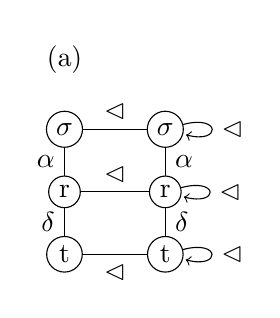
\begin{tikzpicture} [baseline = (x.base)]
\matrix (m) [matrix of nodes, column sep = 1em, row sep = 1em]{
(a) \\
\node[draw,circle, inner sep =2pt](x){$\sigma$}; & &  \node[draw,circle, inner sep =2pt](x2){$\sigma$};\\
\node[draw,circle, inner sep =2pt](y){r}; & & \node[draw,circle, inner sep =2pt](y2){r};& \\
\node[draw,circle, inner sep =2pt](z){t};  & & \node[draw,circle, inner sep =2pt](z2){t}; & \\
};
\draw (x) -- (y) node[left, pos=.5]{$\alpha$};
\draw (z) -- (y) node[left, pos=.5]{$\delta$};
\draw (x2) -- (y2) node[right, pos=.5]{$\alpha$};
\draw (z2) -- (y2) node[right, pos=.5]{$\delta$};
\draw (x) -- (x2) node[above, pos=.5]{$\vartriangleleft$};
\draw (y) -- (y2) node[above, pos=.5]{$\vartriangleleft$};
\draw (z) -- (z2) node[below, pos=.5]{$\vartriangleleft$};
\path (x2) edge [loop right] node{$\vartriangleleft$} (x2);
\path (y2) edge [loop right] node{$\vartriangleleft$} (y2);
\path (z2) edge [loop right] node{$\vartriangleleft$} (z2);
\end{tikzpicture}
\hspace{1em}
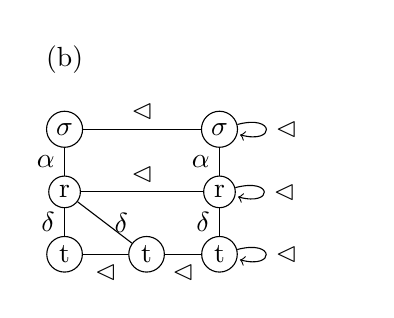
\begin{tikzpicture} [baseline = (x.base)]
\matrix (m) [matrix of nodes, column sep = 1.3em, row sep = 1em]{
(b) \\
\node[draw,circle, inner sep =2pt](x){$\sigma$}; & & \node[draw,circle, inner sep =2pt](x2){$\sigma$};  & & \hspace{1em} \\
\node[draw,circle, inner sep =2pt](y){r}; & & \node[draw,circle, inner sep =2pt](y2){r}; & \\
\node[draw,circle, inner sep =2pt](z){t}; & \node[draw,circle, inner sep =2pt](v){t}; & \node[draw,circle, inner sep =2pt](z2){t};&  \\
};
\draw (x) -- (y) node[left, pos=.5]{$\alpha$};
\draw (z) -- (y) node[left, pos=.5]{$\delta$};
\draw (v) -- (y) node [right, pos =.5]{$\delta$};
\draw (x2) -- (y2) node[left, pos=.5]{$\alpha$};
\draw (z2) -- (y2) node[left, pos=.5]{$\delta$};
\draw (x) -- (x2) node[above, pos=.5]{$\vartriangleleft$};
\draw (y) -- (y2) node[above, pos=.5]{$\vartriangleleft$};
\draw (z) -- (v) node[below, pos=.5]{$\vartriangleleft$};
\draw (v) -- (z2) node[below, pos=.5]{$\vartriangleleft$};
\path (x2) edge [loop right] node{$\vartriangleleft$} (x2);
\path (y2) edge [loop right] node{$\vartriangleleft$} (y2);
\path (z2) edge [loop right] node{$\vartriangleleft$} (z2);
\end{tikzpicture}
\hspace{1em}
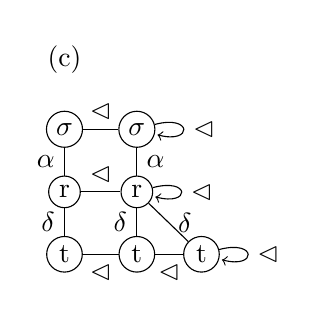
\begin{tikzpicture} [baseline = (x.base)]
\matrix (m) [matrix of nodes, column sep = 1em, row sep = 1em]{
(c) \\
\node[draw,circle, inner sep =2pt](x){$\sigma$}; &  \node[draw,circle, inner sep =2pt](x2){$\sigma$}; \\
\node[draw,circle, inner sep =2pt](y){r}; &  \node[draw,circle, inner sep =2pt](y2){r}; \\
\node[draw,circle, inner sep =2pt](z){t};  & \node[draw,circle, inner sep =2pt](z2){t};  &\node[draw,circle, inner sep =2pt](v2){t}; \\
};
\draw (x) -- (y) node[left, pos=.5]{$\alpha$};
\draw (z) -- (y) node[left, pos=.5]{$\delta$};
\draw (x2) -- (y2) node[right, pos=.5]{$\alpha$};
\draw (z2) -- (y2) node[left, pos=.5]{$\delta$};
\draw (v2) -- (y2) node [right, pos =.5]{$\delta$};
\draw (x) -- (x2) node[above, pos=.5]{$\vartriangleleft$};
\draw (y) -- (y2) node[above, pos=.5]{$\vartriangleleft$};
\draw (z) -- (z2) node[below, pos=.5]{$\vartriangleleft$};
\draw (z2) -- (v2) node[below, pos=.5]{$\vartriangleleft$};
\path (x2) edge [loop right] node{$\vartriangleleft$} (x2);
\path (y2) edge [loop right] node{$\vartriangleleft$} (y2);
\path (v2) edge [loop right] node{$\vartriangleleft$} (v2);
\end{tikzpicture}
\hspace{1em}
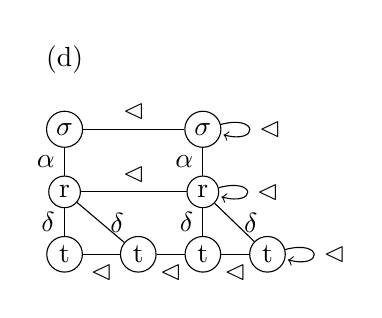
\begin{tikzpicture} [baseline = (x.base)]
\matrix (m) [matrix of nodes, column sep = 1em, row sep = 1em]{
(d) \\
\node[draw,circle, inner sep =2pt](x){$\sigma$}; & & \node[draw,circle, inner sep =2pt](x2){$\sigma$}; \\
\node[draw,circle, inner sep =2pt](y){r}; & & \node[draw,circle, inner sep =2pt](y2){r}; \\
\node[draw,circle, inner sep =2pt](z){t}; & \node[draw,circle, inner sep =2pt](v){t}; & \node[draw,circle, inner sep =2pt](z2){t}; &  \node[draw,circle, inner sep =2pt](v2){t}; \\
};
\draw (x) -- (y) node[left, pos=.5]{$\alpha$};
\draw (z) -- (y) node[left, pos=.5]{$\delta$};
\draw (v) -- (y) node [right, pos =.5]{$\delta$};
\draw (x2) -- (y2) node[left, pos=.5]{$\alpha$};
\draw (z2) -- (y2) node[left, pos=.5]{$\delta$};
\draw (v2) -- (y2) node [right, pos =.5]{$\delta$};
\draw (x) -- (x2) node[above, pos=.5]{$\vartriangleleft$};
\draw (y) -- (y2) node[above, pos=.5]{$\vartriangleleft$};
\draw (z) -- (v) node[below, pos=.5]{$\vartriangleleft$};
\draw (v) -- (z2) node[below, pos=.5]{$\vartriangleleft$};
\draw (z2) -- (v2) node[below, pos=.5]{$\vartriangleleft$};
\path (x2) edge [loop right] node{$\vartriangleleft$} (x2);
\path (y2) edge [loop right] node{$\vartriangleleft$} (y2);
\path (v2) edge [loop right] node{$\vartriangleleft$} (v2);
\end{tikzpicture} \\
Let us examine each in turn. In (a), Axioms I and IV are satisfied by virtue of the association and dominance relations holding between TBU-register and register-terminal pairs only. The first elements of each are in these respective relations, thereby satisfying Axioms II and IV. The first TBU-register pair adheres to Axiom III, since their successors are also in the association relation. The same is true for the final pair given the definition of successor. Axiom VI is satisfied by both register-terminal pairs (much like the TBU-register pairs) via the first disjunct. Axioms I-V are satisfied by the remainder of (b), (c), and (d), but the definition of Axiom VI is worth some further discussion with respect to possible combinations of level and contour tones in these examples. The first disjunct of this axiom defines configurations in which the respective successors of two elements which are in the dominance relation will also be in the dominance relation. Register-terminal pairs in several positions satisfy Axiom VI via this disjunct. This includes a level tone followed by any level tone (as in (a)), a level tone and the first terminal node of a contour (as in (c)), the rightmost terminal node of a contour and a level tone (as in (b)), the rightmost node of a contour and the leftmost node of a following contour (as in (d)), and the final register-terminal pair in either level or contour tones ((a)-(d)). What remains to be described is an important structural position, that is, the leftmost terminal node in a contour. The second disjunct in Axiom VI is satisfied by register-terminal pairs for which the terminal is the leftmost node in a contour tone. Here, the conjunct $\delta(succ(x)) \ap y$ establishes a sisterhood relationship between `t' nodes in a contour (dominated by the same register node). The second conjunct $\delta(succ(succ(x)))\ap succ(y)$ imposes an upper bound on register node branching, setting the limit at two terminal nodes per root. In other words, the immediate successor of a terminal node can be dominated by the same register node (forming a contour), but the successor of that node must be dominated by the following register node. 
\subsection{Bao (1990)}
Bao (1990) explores the empirical behavior of tone cross-linguistically and examines the formal relations between tone and other phonological structures to propose a novel tonal geometry. This representation conceptualizes tone as a separate tier on the syllable plane (associating to a TBU via adjunction), but not a separate plane itself. The internal structure of tone differs crucially from Yip's model in two ways. First, the tonal root node and register node (conflated in Yip's tonal geometry) are separate nodes. The root node `T' (`t' in the original, but capitalized here to distinguish it from terminal tonal `t' nodes in our terminology) \emph{dominates} a separate register node which is specified by the laryngeal feature [$\pm$stiff]. This feature is equivalent to Yip's [$\pm$upper] in that it divides the vocal range into two registers. The root node further dominates a `c' or `contour' node which dominates up to two terminal tonal nodes, specified [$\pm$slack] in Bao's terms.\footnote{Bao's representation has register as a non-terminal `r' node which dominates the feature [$\pm$stiff]. However, he mentions that it is non-branching, and in his representation the domination is indicated by a dotted line. Later, in Chen (2000), the position of the `r' node is precisely the terminal register feature node, that is, directly dominated by the root `T'. I abstract away from this detail here and use the representation from Chen (2000).}
\begin{center}
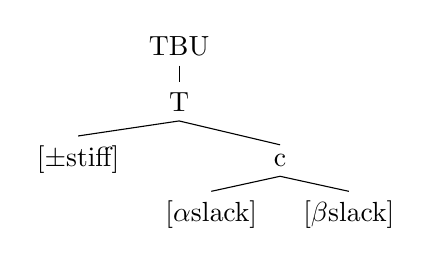
\begin{tikzpicture}[baseline = (current bounding box.north), sibling distance = 10pt]
\tikzset{level distance = 20pt}
\Tree [.TBU [.T [.{$[\pm$stiff$]$} ] [.c [.{$[\alpha$slack$]$} ] [.{$[\beta$slack$]$} ]]]];
\end{tikzpicture}
\end{center}
Much like Yip's [$\pm$raised] feature, sequences of [$\pm$slack] are used to denote rising and falling contours, with single nodes denoting level tones. Bao offers only the formal configuration of `c' terminal nodes above. An implicit upper bound of two on `c' node branching is thus implicit in his model. \par
We can explicitly define structures in Bao's tonal geometry by defining models over them. Identical to those defined over Yip's representation, these models comprise domains of elements corresponding to nodes in Bao's configuration: syllable TBUs, root `T' nodes, register nodes, `c' nodes, and terminal tonal nodes. These elements are assigned a label (designating node type or feature) with a set of unary functions. Binary functions define relations between elements which mimic association, domination (internal structure of tones) and linear order in Bao's tonal representation. We define a signature $\zeta_{b}$ for the relations and functions in a Bao model. To highlight the equivalencies between Yip and Bao representations, Bao's [$\pm$stiff] nodes are defined as [$\pm$u], [+slack] as `h', and [-slack] as `l': 
\begin{equation}
\zeta_{b}\myeq \{P_{\sigma}, P_{T}, P_{+u}, P_{-u}, P_{h}, P_{l}, P_{c}; \alpha, \delta, succ\} \\
\end{equation}
This signature contains seven unary relations which label domain elements as one of syllable, `T' root, register ($P_{+u}$, $P_{-u}$), `c', or terminal tonal ($P_{h}$, $P_{l}$) nodes. Identical to Yip's model, three binary functions specify the association relation between a TBU and tonal root ($\alpha$), dominance relations between `T'-c, `T'-register, and c-terminal node pairs ($\delta$), as well as linear order on intra-tier elements ($succ$). \par
We illustrate with an example of a model of a Zhenhai structure. The Zhenhai word  \textipa{f\~a}$^{11}$ \textipa{k\;E}$^{334}$ [L.MH] `bedroom' can be represented in Bao's terms as follows: two syllables associate to respective tonal root `T' nodes; the leftmost `T' node dominates a register node (specified as [-stiff]) and a `c' node, the latter of which dominates a terminal [+slack] node. The rightmost root node dominates a [+stiff] register node and a `c' node which itself dominates a sequence of two terminal nodes. These are specified [+slack] and [-slack], respectively to indicate a rising contour.
\begin{center}
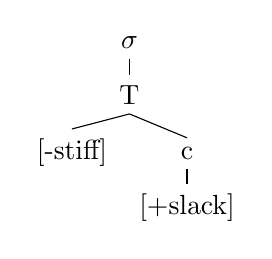
\begin{tikzpicture}[baseline = (current bounding box.north), sibling distance = 5pt]
\tikzset{level distance = 20pt}
\Tree [.$\sigma$ [.T [.{$[$-stiff$]$} ] [.c [.{$[$+slack$]$} ] ]]];
\end{tikzpicture}
\hspace{1em}
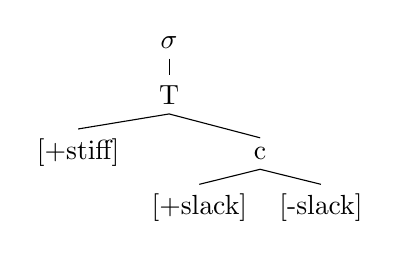
\begin{tikzpicture}[baseline = (current bounding box.north), sibling distance = 5pt]
\tikzset{level distance = 20pt}
\Tree [.$\sigma$ [.T [.{$[$+stiff$]$} ] [.c [.{$[$+slack$]$} ] [.{$[$-slack$]$} ]]]];
\end{tikzpicture}
\end{center}
Let $\mathcal{M}^{B}_{zh}$ be a model over a domain of elements, labeled and related to one another via a set of relations and functions. Recall that, as indicated above, an equivalency holds between Yip's [upper] and Bao's [stiff], Yip's [-raised] and Bao's [+slack], and Yip's [+raised] and Bao's [-slack]. The model is defined below.
\begin{equation}
\begin{aligned}
\mathcal{M}^{B}_{zh} \myeq \langle \mathcal{D}; &P_{\sigma}, P_{T}, P_{+u}, P_{-u}, P_{h}, P_{l}, P_{c}; \\
\alpha(x)\ap y, &\delta(x)\ap y, succ(x)\ap y \rangle \\
\mathcal{D} &= \{1, 2, 3, 4, 5, 6, 7, 8, 9, 10, 11\}  \\
P_{\sigma} &= \{1, 2\} & P_{T} &= \{3, 4\} \\
P_{+u} &= \{7\} & P_{-u} &= \{5\} \\
P_{h} &= \{11\} & P_{l} &= \{9, 10\} \\ 
P_{c} &= \{6, 8\}& \alpha(x)\ap y &= \begin{cases} 3 & x=1 \\ 4 & x=2 \end{cases}  \\
 \delta(x)\ap y &= \begin{cases} 3 & x\in\{5,6\} \\ 4 & x\in \{7,8\} \\ 6 & x=9 \\ 8 & x\in\{10,11\} \end{cases} &
succ(x)\ap y &= \begin{cases} 2 & x\in \{1,2\} \\ 4 & x\in \{3,4\} \\ 7 & x\in\{5,7\} \\ 8 & x\in\{6,8\} \\ 10 & x=9 \\ 11 & x\in\{10,11\} \end{cases} \\
\end{aligned}
\end{equation}
Graphically, the model $\mathcal{M}^{B}_{zh}$ can be represented as:
\begin{center}
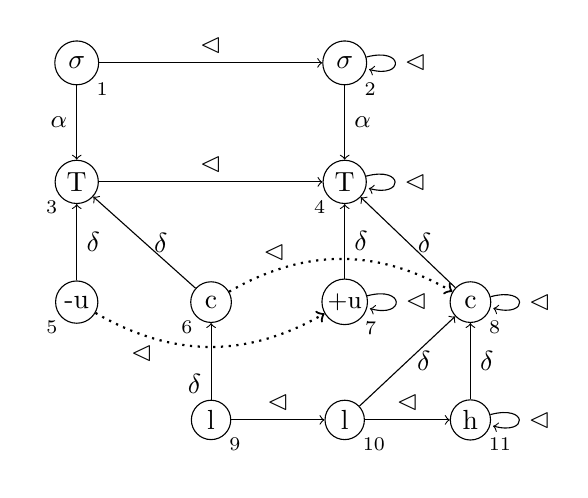
\begin{tikzpicture} [baseline = (x.base)]
\matrix (m) [matrix of nodes, column sep = 2em, row sep = 2em]{
\node[draw,circle, inner sep =3pt, label ={[label distance = -3pt] below right:\scriptsize1}](x){$\sigma$}; & &  \node[draw,circle, inner sep =3pt, label ={[label distance = -3pt] below right:\scriptsize2}](x2){$\sigma$};\\
\node[draw,circle, inner sep =2pt, label ={[label distance = -3pt] below left:\scriptsize3}](y){T}; & & \node[draw,circle, inner sep =2pt, label ={[label distance = -3pt] below left:\scriptsize4}](y2){T};& \\
\node[draw,circle, inner sep =2pt, label ={[label distance = -3pt] below left:\scriptsize5}](z){-u};  & \node[draw,circle, inner sep =3pt, label ={[label distance = -3pt] below left:\scriptsize6}](z1){c}; & \node[draw,circle, inner sep =1pt, label ={[label distance = -3pt] below right:\scriptsize7}](z2){\se u}; & \node[draw,circle, inner sep =3pt, label ={[label distance = -3pt] below right:\scriptsize8}](z3){c}; \\
& \node[draw,circle, inner sep =2.5pt, label ={[label distance = -3pt] below right:\scriptsize9}](t1){l}; & \node[draw,circle, inner sep =2.5pt, label ={[label distance = -3pt] below right:\scriptsize10}](t2){l}; & \node[draw,circle, inner sep =2pt, label ={[label distance = -3pt] below right:\scriptsize11}](t3){h}; \\
};
\draw [->](x) -- (y) node[left, pos=.5]{\small$\alpha$};
\draw [->](z) -- (y) node[right, pos=.5]{$\delta$};
\draw [->](z1) -- (y) node[right, pos=.5]{$\delta$};
\draw [->](x2) -- (y2) node[right, pos=.5]{\small$\alpha$};
\draw [->](z2) -- (y2) node[right, pos=.5]{$\delta$};
\draw [->](t1) -- (z1) node[left, pos=.2]{$\delta$};
\draw [->](t2) -- (z3) node[right, pos=.5]{$\delta$};
\draw [->](t3) -- (z3) node[right, pos=.5]{$\delta$};
\draw [->](z3) -- (y2) node[right, pos=.5]{$\delta$};
\draw [->](x) -- (x2) node[above, pos=.5]{$\vartriangleleft$};
\draw [->](t1) -- (t2) node[above, pos=.5]{$\vartriangleleft$};
\draw [->](t2) -- (t3) node[above, pos=.5]{$\vartriangleleft$};
\draw [->](y) -- (y2) node[above, pos=.5]{$\vartriangleleft$};
\path (x2) edge [loop right] node{$\vartriangleleft$} (x2);
\path (y2) edge [loop right] node{$\vartriangleleft$} (y2);
\path (z3) edge [loop right] node{$\vartriangleleft$} (z3);
\path (z2) edge [loop right] node{$\vartriangleleft$} (z2);
\path (t3) edge [loop right] node{$\vartriangleleft$} (t3);
\path [thick, dotted, ->] (z) edge [bend right=30] node[below,pos=.2]{$\vartriangleleft$} (z2);
\path [thick, dotted, ->] (z1) edge [bend left=30] node[above,pos=.2]{$\vartriangleleft$} (z3);
\end{tikzpicture}
\end{center}
The model $\mathcal{M}^{B}_{zh}$ is defined over a set of domain elements of size 11. The unary relation $P_{\sigma}(x)$ labels elements 1 and 2 as syllables, which form the TBU syllable nodes. Elements 3 and 4 are labeled as tonal root nodes by $P_{T}(x)$. The definition of the binary function $\alpha(x)\ap y$ specifies a relation between elements 1-3 and 2-4, representing TBU-to-tone (root) association (recall that this relation held between syllables and \emph{register} nodes in Yip's model). Register and `c' nodes are labeled via the relations $P_{+u}(x)$/$P_{-u}(x)$ and $P_{c}$, respectively; element 5 acquires a [-u] label, element 7 a [+u] label, and elements 6 and 8 both acquire `c' labels. The first two cases of the $\delta(x)\ap y$ definition establish dominance relations between elements 5,6 and 3, and elements 7,8 and 4, such that 5 and 6 are immediately dominated by 3, and 7 and 8 are immediately dominated by 4. These cases reflect Bao's crucial notion of \emph{separate register and contour nodes} dominated by a tonal root. The remaining elements (9-11) are labeled appropriately as terminal tonal nodes via $P_{h}(x)$ and $P_{l}(x)$, and enter into a dominance relation with the `c' nodes (elements 6 and 8) in the last three cases of the $\delta(x)\ap y$ definition. Note that in the Yip model, terminal root nodes are immediately dominated by \emph{register} nodes. In summary, the domain elements 1,3,5,6,9 and their respective relational definitions model the first syllable \textipa{f\~a}$^{11}$ (a low-registered low tone [L]); elements 2,4,7,8,10,11 and their relational definitions model the second syllable \textipa{k\;E}$^{334}$ (a high-registered rising tone [MH]). Similar to the Yip model, the successor function ($succ(x)\ap y$) establishes linear order over the model elements on the same tier; the [L] syllable is succeeded by the [MH] syllable, and the contour is rising (not falling). Note that no ordering is defined over register and `c' nodes; this reflects Bao's generalization that these nodes are not ordered with respect to one another (in spite of their sisterhood), such that the following forms are equivalent:
\begin{center}
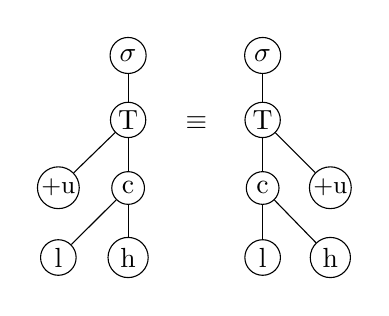
\begin{tikzpicture} [baseline = (x1.base)]
\matrix (m) [matrix of nodes, column sep = 1em, row sep = 1em]{
& \node[draw,circle, inner sep =2pt](x1){$\sigma$}; & &  \node[draw,circle, inner sep =2pt](x2){$\sigma$};  \\
& \node[draw,circle, inner sep =1pt](y1){T};  & $\equiv$ & \node[draw,circle, inner sep =1pt](y2){T}; \\
\node[draw,circle, inner sep =.5pt](z1){\se u}; & \node[draw,circle, inner sep =2pt](z2){c}; & &  \node[draw,circle, inner sep =2pt](z3){c}; & \node[draw,circle, inner sep =.5pt](z4){\se u}; \\
\node[draw,circle, inner sep =2pt](t1){l}; & \node[draw,circle, inner sep =2pt](t2){h}; & &  \node[draw,circle, inner sep =2pt](t3){l}; & \node[draw,circle, inner sep =2pt](t4){h}; \\
};
\draw (x1) -- (y1);
\draw (x2) -- (y2);
\draw (z1) -- (y1);
\draw (z2) -- (y1);
\draw (z2) -- (t1);
\draw (z2) -- (t2);
\draw (y2) -- (z3);
\draw (y2) -- (z4);
\draw (z3) -- (t3);
\draw (z3) -- (t4);
\end{tikzpicture}
\end{center}
Using this model, then, all crucial components of Bao's tonal geometry can be explicitly defined and modeled. \par
The remainder of this section offers a general model theoretic description of Bao's tonal geometry, one which is satisfied by the Zhenhai structure above, but which also generalizes to any tonal structure in Bao's paradigm. \par
Yip's general model is characterized as a three-tiered string sequence. Bao's general model, by contrast, comprises five tiers: TBU's (which we will call syllables), terminal root `T' nodes, register `r' nodes, contour `c' nodes, and terminal tonal nodes `t':
\begin{center}
\begin{tikzpicture}
\matrix (m) [matrix of nodes, column sep = .3em, row sep= 1em]{
 $\sigma$ & $\sigma$ & $\sigma$ & $\dotso$ \\
 T & T & T & $\dotso$ \\
 r & r & r & $\dotso$ \\
 c & c & c & $\dotso$ \\
 t & t & t & $\dotso$ \\
};
\end{tikzpicture}
\end{center}
String labeling is determined via unary relations in the same fashion as the Yip model, but with the addition of unary relations which label tonal root `T' nodes and contour `c' nodes. Relations between nodes are also governed by the same three binary functions, however, their definitions differ. The association function ($\alpha(x)\ap y$) takes a syllable TBU node and outputs a tautosyllabic root node; this node, however, is not specified for register features, but rather is an independent root `T' node. Dominance relations are comparatively more complex in the Bao model, as well. Within a syllable, the function $\delta(x)\ap y$ takes either a register or `c' node and outputs the root `T' node which serves as the immediate dominator. Additionally, the function is defined as a terminal root node in the domain, and the tautosyllabic `c' node in the codomain. There are thus two levels of dominance. Like Yip's model, a successor function is defined over elements of the five tiers (but not between them) thus establishing linear order. An important detail about this ordering is that while register and `c' nodes are sisters under the same `T' node (that is, they are on a `tier' with respect to dominance), there is no linear order between them. The successor function in Bao's model is also total such that the final element in a tier is its own successor. The relations and functions described here define relations between Bao model elements for any structure using Bao's representation. \par
We define a series of axioms which govern relations between domain elements in the Bao model, also utilizing the auxiliary relations defined in (\ref{aux1}) and (\ref{aux2}). We begin with association.
\begin{equation}
\begin{aligned}
&\text{AxI:}\,(\all x,y)[\alpha(x)\ap y \rightarrow P_{\sigma}(x)\land P_{T}(y)]\\
&\text{AxII:}\,(\all x,y)[(first_{\sigma}(x)\land first_{T}(y))\rightarrow\alpha(x)\ap y]\\
&\text{AxIII:}\,(\all x,y)[\alpha(x) \ap y \rightarrow \alpha(succ(x))\ap succ(y)] \\
\end{aligned}
\end{equation}
Note that axioms I-III are identical across both models with the exception of the featural label of the function's co-domain; Yip's tonal root is the register node, while Bao's tonal root is the `T' node. Again, these axioms ensure association between syllable and `T' root nodes in a one-to-one fashion. Axiom I specifies the labeled elements which enter into the relation, while Axioms II and III limit association to tautosyllabic nodes, beginning with the first element of the relevant tiers. \par
Dominance in Bao's model is a bit more complex, because the relation holds between more than two categories of nodes. There are three distinct instances of dominance that need to be captured in the definition. We offer three axioms governing dominance.
\begin{equation}
\begin{aligned}
&\text{AxIV:}\,(\all x,y)[\delta(x)\ap y \rightarrow \big((P_{r}(x)\land P_{T}(y))\,\lor \\
&\quad (P_{c}(x)\land P_{T}(y)) \lor (P_{t}(x)\land P_{c}(y))\big)] \\
&\text{AxV:}\,(\all x,y)[\big((first_{r}(x)\land first_{T}(y)) \,\lor \\
&\quad (first_{c}(x)\land first_{T}(y))\lor (first_{t}(x)\,\land \\
&\quad first_{c}(y))\big) \rightarrow \delta(x) \ap y] \\
&\text{AxVI:}\,(\all x,y)[\delta(x)\ap y \rightarrow \Big(\big(P_{r}(x)\land P_{T}(y)\,\land \\
&\quad \delta(succ(x)) \ap succ(y)\big) \lor \big(P_{c}(x)\land P_{T}(y)\,\land \\
&\quad \delta(succ(x)) \ap succ(y)\big)\lor \big(P_{t}(x)\land P_{c}(y) \,\land \\
&\quad (\delta(succ(x))\ap succ(y)\lor (\delta(succ(x))\ap y \,\land \\
&\quad \delta(succ(succ(x)))\ap succ(y)))\big)\Big)] \\
\end{aligned}
\end{equation}
Axiom IV specifies which types of nodes can enter into the dominance relation. Dominance here implies that either a register node is dominated by a root `T' node, a `c' node is dominated a `T' node, or that a terminal `t' node is dominated by a `c' node \emph{and nothing else}. Axiom V establishes a dominance relationship between string-initial elements in the corresponding string pairs described above (r-T, c-T, t-c). Finally, Axiom VI restricts the scope of dominance to tautosyllabic nodes. The consequent of this axiom comprises three disjuncts, each of which governs dominance between a specific string pair. Each disjunct is made of three conjuncts. The first two specify string pair labels, and the third defines how dominance proceeds, whether it is one-to-one (in the case of r-T and c-T pairs) or one-to-one with the option of two-to-one dominance (for t-c pairs). Note that the basic structure of these axioms is identical to those proposed for the Yip model, with a few extensions to accommodate dominance between multiple string pairs. While it is possible to collapse the definition of Axiom IV into Axiom VI, the purpose of defining the axioms as they appear above is to highlight the parallels between the two models. \par
Consider the four examples below which exhaust the logically-possible combinations of level contour tones in Bao's model. For the convenience of the reader, successor relations are omitted. Note that the Zhenhai example is of basic type (b).\\
\noindent
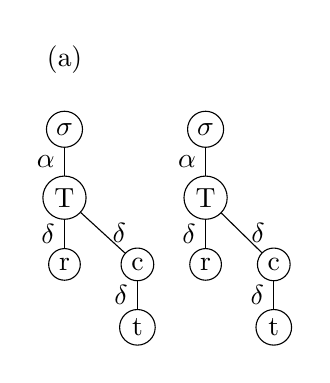
\begin{tikzpicture} [baseline = (x.base)]
\matrix (m) [matrix of nodes, column sep = 1em, row sep = 1em]{
(a) \\
\node[draw,circle, inner sep =2pt](x){$\sigma$}; & & \node[draw,circle, inner sep =2pt](x2){$\sigma$}; \\
\node[draw,circle, inner sep =2pt](y){T}; & & \node[draw,circle, inner sep =2pt](y2){T}; \\
\node[draw,circle, inner sep =2pt](z){r}; & \node[draw,circle, inner sep =2pt](v){c}; & \node[draw,circle, inner sep =2pt](z2){r}; &  \node[draw,circle, inner sep =2pt](v2){c}; \\
 & \node[draw,circle, inner sep =2pt](t2){t}; &  & \node[draw,circle, inner sep =2pt](t4){t}; \\
};
\draw (x) -- (y) node[left, pos=.5]{$\alpha$};
\draw (z) -- (y) node[left, pos=.5]{$\delta$};
\draw (v) -- (y) node [right, pos =.5]{$\delta$};
\draw (x2) -- (y2) node[left, pos=.5]{$\alpha$};
\draw (z2) -- (y2) node[left, pos=.5]{$\delta$};
\draw (v2) -- (y2) node [right, pos =.5]{$\delta$};
\draw (t2) -- (v) node[left, pos=.5]{$\delta$};
\draw (t4) -- (v2) node[left, pos=.5]{$\delta$};
\end{tikzpicture}
\hspace{.25cm}
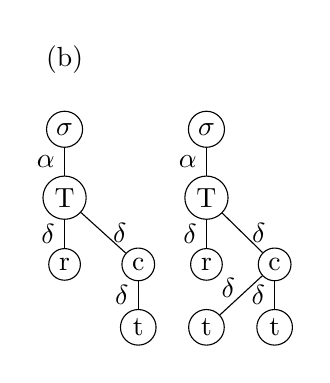
\begin{tikzpicture} [baseline = (x.base)]
\matrix (m) [matrix of nodes, column sep = 1em, row sep = 1em]{
(b) \\
\node[draw,circle, inner sep =2pt](x){$\sigma$}; & & \node[draw,circle, inner sep =2pt](x2){$\sigma$}; \\
\node[draw,circle, inner sep =2pt](y){T}; & & \node[draw,circle, inner sep =2pt](y2){T}; \\
\node[draw,circle, inner sep =2pt](z){r}; & \node[draw,circle, inner sep =2pt](v){c}; & \node[draw,circle, inner sep =2pt](z2){r}; &  \node[draw,circle, inner sep =2pt](v2){c}; \\
& \node[draw,circle, inner sep =2pt](t2){t}; & \node[draw,circle, inner sep =2pt](t3){t}; & \node[draw,circle, inner sep =2pt](t4){t}; \\
};
\draw (x) -- (y) node[left, pos=.5]{$\alpha$};
\draw (z) -- (y) node[left, pos=.5]{$\delta$};
\draw (v) -- (y) node [right, pos =.5]{$\delta$};
\draw (x2) -- (y2) node[left, pos=.5]{$\alpha$};
\draw (z2) -- (y2) node[left, pos=.5]{$\delta$};
\draw (v2) -- (y2) node [right, pos =.5]{$\delta$};
\draw (t2) -- (v) node[left, pos=.5]{$\delta$};
\draw (t3) -- (v2) node[above, pos=.2]{$\delta$};
\draw (t4) -- (v2) node[left, pos=.5]{$\delta$};
\end{tikzpicture}
\hspace{.25cm}
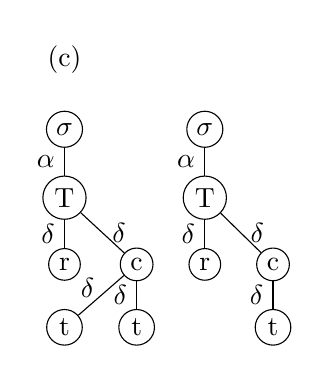
\begin{tikzpicture} [baseline = (x.base)]
\matrix (m) [matrix of nodes, column sep = 1em, row sep = 1em]{
(c) \\
\node[draw,circle, inner sep =2pt](x){$\sigma$}; & & \node[draw,circle, inner sep =2pt](x2){$\sigma$}; \\
\node[draw,circle, inner sep =2pt](y){T}; & & \node[draw,circle, inner sep =2pt](y2){T}; \\
\node[draw,circle, inner sep =2pt](z){r}; & \node[draw,circle, inner sep =2pt](v){c}; & \node[draw,circle, inner sep =2pt](z2){r}; &  \node[draw,circle, inner sep =2pt](v2){c}; \\
\node[draw,circle, inner sep =2pt](t1){t}; & \node[draw,circle, inner sep =2pt](t2){t}; &  & \node[draw,circle, inner sep =2pt](t4){t}; \\
};
\draw (x) -- (y) node[left, pos=.5]{$\alpha$};
\draw (z) -- (y) node[left, pos=.5]{$\delta$};
\draw (v) -- (y) node [right, pos =.5]{$\delta$};
\draw (x2) -- (y2) node[left, pos=.5]{$\alpha$};
\draw (z2) -- (y2) node[left, pos=.5]{$\delta$};
\draw (v2) -- (y2) node [right, pos =.5]{$\delta$};
\draw (t1) -- (v) node[above, pos=.2]{$\delta$};
\draw (t2) -- (v) node[left, pos=.5]{$\delta$};
\draw (t4) -- (v2) node[left, pos=.5]{$\delta$};
\end{tikzpicture}
\hspace{.4cm}
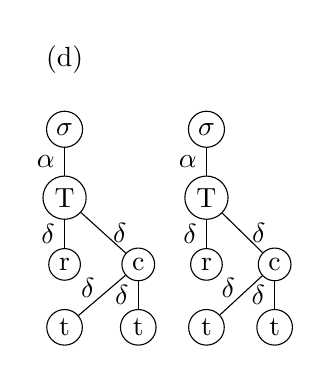
\begin{tikzpicture} [baseline = (x.base)]
\matrix (m) [matrix of nodes, column sep = 1em, row sep = 1em]{
(d) \\
\node[draw,circle, inner sep =2pt](x){$\sigma$}; & & \node[draw,circle, inner sep =2pt](x2){$\sigma$}; \\
\node[draw,circle, inner sep =2pt](y){T}; & & \node[draw,circle, inner sep =2pt](y2){T}; \\
\node[draw,circle, inner sep =2pt](z){r}; & \node[draw,circle, inner sep =2pt](v){c}; & \node[draw,circle, inner sep =2pt](z2){r}; &  \node[draw,circle, inner sep =2pt](v2){c}; \\
\node[draw,circle, inner sep =2pt](t1){t}; & \node[draw,circle, inner sep =2pt](t2){t}; & \node[draw,circle, inner sep =2pt](t3){t}; & \node[draw,circle, inner sep =2pt](t4){t}; \\
};
\draw (x) -- (y) node[left, pos=.5]{$\alpha$};
\draw (z) -- (y) node[left, pos=.5]{$\delta$};
\draw (v) -- (y) node [right, pos =.5]{$\delta$};
\draw (x2) -- (y2) node[left, pos=.5]{$\alpha$};
\draw (z2) -- (y2) node[left, pos=.5]{$\delta$};
\draw (v2) -- (y2) node [right, pos =.5]{$\delta$};
\draw (t1) -- (v) node[above, pos=.2]{$\delta$};
\draw (t2) -- (v) node[left, pos=.5]{$\delta$};
\draw (t3) -- (v2) node[above, pos=.2]{$\delta$};
\draw (t4) -- (v2) node[left, pos=.5]{$\delta$};
\end{tikzpicture} \\
Similar to Yip's model, the association relations in (a)-(d) satisfy the first three axioms. Association obtains between syllable and root `T' nodes only (Axiom I), the first element in each of the two strings associates (Axiom II), and the successor of each string pair also associates (Axiom III). Again, given that the successor function is a total function, the final syllable-root string pair also satisfies Axiom III. Any configuration in a Bao model with one-to-one association between syllable and root `T' nodes will satisfy these axioms. \par
The dominance relation that holds between r-T and c-T pairs is uniform across examples (a)-(d). These relations satisfy Axioms IV and V in much the same way as the association relations satisfy Axioms I and II, that is, the proper nodes are in the relation, and the first element of the string pairs is in the relation. Additionally, the r-T and c-T pairs satisfy Axiom VI via the first two disjuncts of the consequent, as the successors of all r-T and c-T pairs are in the dominance relation. \par
Note that the third disjunct of the consequent in Axiom IV ($P_{t}(x)\land P_{c}(y)$), the third disjunct of the antecedent in Axiom V ($first_{t}(x)\land first_{c}(y)$), and the second conjunct of the consequent's final disjunct in Axiom VI ($\delta(succ(x))\ap succ(y)\lor (\delta(succ(x))\ap y \land \delta(succ(succ(x)))\ap succ(y))$) are identical to Axioms IV, V, and VI in Yip's model with the exception that the `r' node in Yip's model is equivalent to the `c' node in Bao's model. The t-c pairs which form the logically possible combinations of level and contour tones in (a)-(d) therefore satisfy Axioms IV-VI by the same principles.\par
Structures (a)-(d) in the above figure do not explicitly show the ordering relation on elements in Bao's representation. We offer a final figure with the full specification of the successor function on elements in the Bao model (dominance and association are represented by dotted lines). Crucial to note here is that no ordering is imposed between `r' and `c' nodes, in spite of the fact that they are sisters under a `T' node.
\begin{center}
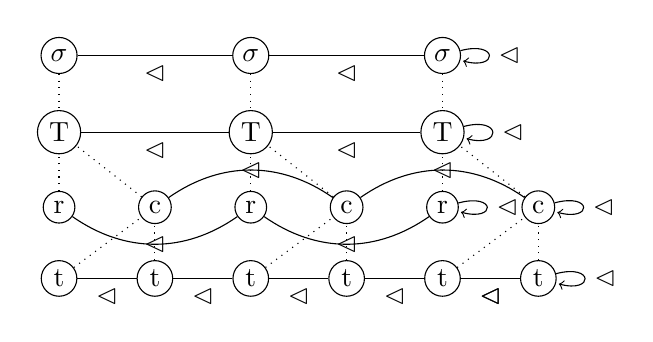
\begin{tikzpicture} [baseline = (x.base)]
\matrix (m) [matrix of nodes, column sep = 2em, row sep = 1.3em]{
\node[draw,circle, inner sep =2pt](x){$\sigma$}; & & \node[draw,circle, inner sep =2pt](x2){$\sigma$}; & & \node[draw,circle, inner sep =2pt](x3){$\sigma$};  \\
\node[draw,circle, inner sep =2pt](y){T}; & & \node[draw,circle, inner sep =2pt](y2){T}; & & \node[draw,circle, inner sep =2pt](y3){T};  \\
\node[draw,circle, inner sep =2pt](z){r}; & \node[draw,circle, inner sep =2pt](v){c}; & \node[draw,circle, inner sep =2pt](z2){r}; & \node[draw,circle, inner sep =2pt](v2){c}; & \node[draw,circle, inner sep =2pt](z3){r}; & \node[draw,circle, inner sep =2pt](v3){c};\\
\node[draw,circle, inner sep =2pt](q){t}; & \node[draw,circle, inner sep =2pt](s){t}; & \node[draw,circle, inner sep =2pt](q2){t}; & \node[draw,circle, inner sep =2pt](s2){t}; & \node[draw,circle, inner sep =2pt](q3){t}; & \node[draw,circle, inner sep =2pt](s3){t}; \\
};
\draw [dotted] (x) -- (y);
\draw [dotted] (z) -- (y);
\draw [dotted] (v) -- (y);
\draw [dotted] (q) -- (v);
\draw [dotted] (s) -- (v);
\draw (q) -- (s) node[below, pos=.5]{$\vartriangleleft$};
\draw [dotted] (x2) -- (y2);
\draw [dotted] (z2) -- (y2);
\draw [dotted] (v2) -- (y2);
\draw [dotted] (q2) -- (v2);
\draw [dotted] (s2) -- (v2);
\draw (q2) -- (s2) node[below, pos=.5]{$\vartriangleleft$};
\draw [dotted] (x3) -- (y3);
\draw [dotted] (z3) -- (y3);
\draw [dotted] (v3) -- (y3);
\draw [dotted] (q3) -- (v3);
\draw [dotted] (s3) -- (v3);
\draw (q3) -- (s3) node[below, pos=.5]{$\vartriangleleft$};
\draw (q3) -- (s3) node[below, pos=.5]{$\vartriangleleft$};
\draw (x) -- (x2) node[below, pos=.5]{$\vartriangleleft$};
\draw (x2) -- (x3) node[below, pos=.5]{$\vartriangleleft$};
\draw (s) -- (q2) node[below, pos=.5]{$\vartriangleleft$};
\draw (s2) -- (q3) node[below, pos=.5]{$\vartriangleleft$};
\path (x3) edge [loop right, align = center] node{$\vartriangleleft$} (x3);
\path (s3) edge [loop right, align = center] node{$\vartriangleleft$} (s3);
\draw (y) -- (y2) node[below, pos=.5]{$\vartriangleleft$};
\draw  (y2) -- (y3) node[below, pos=.5]{$\vartriangleleft$};
\path (y3) edge [loop right, align = center] node{$\vartriangleleft$} (y3);
\path (v) edge [bend left = 35] node{$\vartriangleleft$} (v2);
\path (v2) edge [bend left = 35] node{$\vartriangleleft$} (v3);
\path (v3) edge [loop right, align = center] node{$\vartriangleleft$} (v3);
\path (z) edge [bend right = 35] node{$\vartriangleleft$} (z2);
\path (z2) edge [bend right = 35] node{$\vartriangleleft$} (z3);
\path (z3) edge [loop right, align = center] node{$\vartriangleleft$} (z3);
\end{tikzpicture}
\end{center}
\section{Contour Shift in Zhenhai}
So far, we have highlighted the similarities between the axioms which govern association and dominance in the Yip and Bao models, suggesting some degree of equivalency between the two. In this section, we present a tonal pattern which is purported to be formalizable in one model but not the other. \par
Chen (2000), citing phonetic data from Rose (1990), presents data from Zhenhai, an Wu dialect spoken in Zhenjiang. He argues that Zhenhai sandhi provides evidence for contour shift/spreading independent of register, and therefore motivates separate register and contour nodes in representation. Chen's assessment is that this pattern is predicted by Bao's tonal geometry but not Yip's. \par
Abstracting away from certain details, Chen presents cases of disyllabic sandhi in which the citation contour on an initial syllable appears on a final syllable. An example for \textipa{f\~a}$^{11}$ \textipa{k\;E}$^{334}$ `bedroom' is given below. The H,L,M segments to the right indicate Chen's representational interpretations of Rose's phonetic values. \\
\begin{center}
\begin{tabular}{lllc}
\textipa{f\~a} & \textipa{k\;E} & `bedroom' \\
213 & 441 & base form & /LM.HL/ \\
11 & 334 & sandhi form & [L.MH] \\
\end{tabular}
\end{center}
In Chen's analysis, these forms represent the application of two rules. The first is a \emph{contour shift} which spreads a rising contour from the first syllable to the second syllable.
\begin{center}
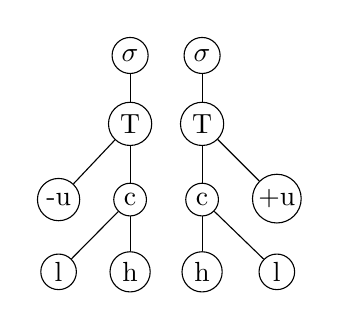
\begin{tikzpicture} [baseline = (y1.base)]
\matrix (m) [matrix of nodes, column sep = 1em, row sep = 1em]{
& \node[draw,circle, inner sep =2pt](x1){$\sigma$};  &  \node[draw,circle, inner sep =2pt](x2){$\sigma$};  \\
& \node[draw,circle, inner sep =2pt](y1){T}; &   \node[draw,circle, inner sep =2pt](y2){T}; \\
\node[draw,circle, inner sep =2pt](z1){-u}; & \node[draw,circle, inner sep =2pt](z2){c}; &   \node[draw,circle, inner sep =2pt](z3){c}; & \node[draw,circle, inner sep =1pt](z4){+u}; \\
\node[draw,circle, inner sep =2pt](t1){l}; & \node[draw,circle, inner sep =2pt](t2){h}; &  \node[draw,circle, inner sep =2pt](t3){h}; & \node[draw,circle, inner sep =2pt](t4){l}; \\
};
\draw (x1) -- (y1);
\draw (x2) -- (y2);
\draw (z1) -- (y1);
\draw (z2) -- (y1);
\draw (z2) -- (t1);
\draw (z2) -- (t2);
\draw (y2) -- (z3);
\draw (y2) -- (z4);
\draw (z3) -- (t3);
\draw (z3) -- (t4);
\end{tikzpicture}
$\rightarrow$
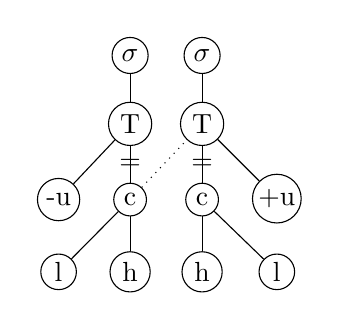
\begin{tikzpicture} [baseline = (y1.base)]
\matrix (m) [matrix of nodes, column sep = 1em, row sep = 1em]{
& \node[draw,circle, inner sep =2pt](x1){$\sigma$};  &  \node[draw,circle, inner sep =2pt](x2){$\sigma$};  \\
& \node[draw,circle, inner sep =2pt](y1){T}; &   \node[draw,circle, inner sep =2pt](y2){T}; \\
\node[draw,circle, inner sep =2pt](z1){-u}; & \node[draw,circle, inner sep =2pt](z2){c}; &   \node[draw,circle, inner sep =2pt](z3){c}; & \node[draw,circle, inner sep =1pt](z4){+u}; \\
\node[draw,circle, inner sep =2pt](t1){l}; & \node[draw,circle, inner sep =2pt](t2){h}; &  \node[draw,circle, inner sep =2pt](t3){h}; & \node[draw,circle, inner sep =2pt](t4){l}; \\
};
\draw (x1) -- (y1);
\draw (x2) -- (y2);
\draw (z1) -- (y1);
\path (z2) edge node{=} (y1);
\draw (z2) -- (t1);
\draw (z2) -- (t2);
\path (z3) edge node{=} (y2);
\draw (y2) -- (z4);
\draw (z3) -- (t3);
\draw (z3) -- (t4);
\draw [dotted] (z2) -- (y2);
\end{tikzpicture}
\end{center}
The second rule is a default `l' insertion rule on the delinked `T' node in the first syllable (hence the low level tone `11' in the output).
\begin{center}
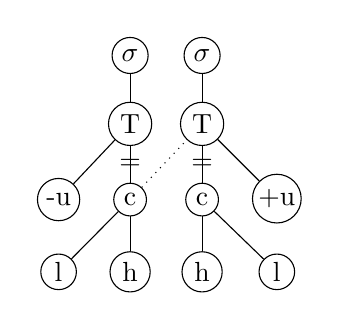
\begin{tikzpicture} [baseline = (y1.base)]
\matrix (m) [matrix of nodes, column sep = 1em, row sep = 1em]{
& \node[draw,circle, inner sep =2pt](x1){$\sigma$};  &  \node[draw,circle, inner sep =2pt](x2){$\sigma$};  \\
& \node[draw,circle, inner sep =2pt](y1){T}; &   \node[draw,circle, inner sep =2pt](y2){T}; \\
\node[draw,circle, inner sep =2pt](z1){-u}; & \node[draw,circle, inner sep =2pt](z2){c}; &   \node[draw,circle, inner sep =2pt](z3){c}; & \node[draw,circle, inner sep =1pt](z4){+u}; \\
\node[draw,circle, inner sep =2pt](t1){l}; & \node[draw,circle, inner sep =2pt](t2){h}; &  \node[draw,circle, inner sep =2pt](t3){h}; & \node[draw,circle, inner sep =2pt](t4){l}; \\
};
\draw (x1) -- (y1);
\draw (x2) -- (y2);
\draw (z1) -- (y1);
\path (z2) edge node{=} (y1);
\draw (z2) -- (t1);
\draw (z2) -- (t2);
\path (z3) edge node{=} (y2);
\draw (y2) -- (z4);
\draw (z3) -- (t3);
\draw (z3) -- (t4);
\draw [dotted] (z2) -- (y2);
\end{tikzpicture}
$\rightarrow$
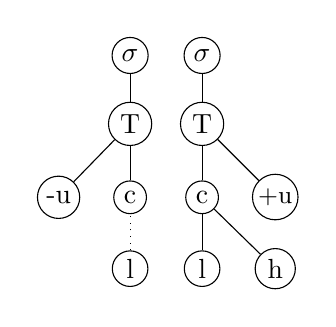
\begin{tikzpicture} [baseline = (y1.base)]
\matrix (m) [matrix of nodes, column sep = 1em, row sep = 1em]{
& \node[draw,circle, inner sep =2pt](x1){$\sigma$};  &  \node[draw,circle, inner sep =2pt](x2){$\sigma$};  \\
& \node[draw,circle, inner sep =2pt](y1){T}; &   \node[draw,circle, inner sep =2pt](y2){T}; \\
\node[draw,circle, inner sep =2pt](z1){-u}; & \node[draw,circle, inner sep =2pt](z2){c}; &   \node[draw,circle, inner sep =2pt](z3){c}; & \node[draw,circle, inner sep =1pt](z4){\se u}; \\
& \node[draw,circle, inner sep =2pt](t1){l}; &  \node[draw,circle, inner sep =2pt](t3){l}; & \node[draw,circle, inner sep =2pt](t4){h}; \\
};
\draw (x1) -- (y1);
\draw (x2) -- (y2);
\draw (z1) -- (y1);
\draw (z2) -- (y1);
\draw (y2) -- (z3);
\draw (y2) -- (z4);
\draw (z3) -- (t3);
\draw (z3) -- (t4);
\draw [dotted] (t1) -- (z2);
\end{tikzpicture}
\end{center}
Important to note here is that \emph{registers} of the syllables do not change. Spreading a rising contour from a low-registered syllable /LM/ ([-u], l-h) to a high-registered syllable /HL/ ([+u], h-l) results in [MH] ([+u], l-h), and crucially \emph{not} [LM]. The key point made by these data is that contour moves independently of register. \par
We can formalize this pattern in an I/O transduction. To do so, we first define two functions (relations?) which identify penults and ultima in a given string:
\begin{equation}
\begin{aligned}
last(x)&\myeq succ(x) = x \\
pnlt(x)&\myeq last(succ(x))\land \neg last(x) \\
\end{aligned}
\end{equation}
Generally speaking, the transduction will represent several `processes'. The first is to spread the `c' node from the penultimate syllable to the final syllable. This will be defined in the output dominance function. In the process, we opt to `delete' the `c' and terminal nodes from the second syllable; this is achieved in the definition of the unary predicates. Finally, the `default l rule' is represented as generation of an additional `l' tone (a `c' node dominating a terminal `l' node) to be dominated by the root node on the penult. For this, we define the transduction over a copy set of size two and generate the low tone in the second copy. \par
We begin by defining the unary relations on the transduction.
\begin{equation} \label{unary}
\begin{aligned}
P^{1}_{\sigma}(x)&\myeq P_{\sigma}(x) & P^{2}_{\sigma}(x)&\myeq \mathtt{False} \\
P^{1}_{T}(x)&\myeq P_{T}(x) & P^{2}_{T}(x)&\myeq \mathtt{False} \\
P^{1}_{-u}(x)&\myeq P_{-u}(x) & P^{2}_{-u}(x)&\myeq \mathtt{False} \\
P^{1}_{+u}(x)&\myeq P_{+u}(x) & P^{2}_{+u}(x)&\myeq \mathtt{False} \\
P^{1}_{c}(x)&\myeq P_{c}(x)\land pnlt(x) & P^{2}_{c}(x)&\myeq P_{c}(x)\land pnlt(x) \\
P^{1}_{h}(x)&\myeq P_{h}(x)\land & P^{2}_{h}(x)&\myeq \mathtt{False} \\
&\quad pnlt(\delta(x)) \\
P^{1}_{l}(x)&\myeq P_{l}(x)\land  & P^{2}_{l}(x)&\myeq P_{l}(x)\land \\
&\quad pnlt(\delta(x)) & &\quad pnlt(\delta(x)) \\
\end{aligned}
\end{equation}
These definitions achieve several goals. First, they preserve syllable, tonal root `T', and register nodes from the input. The relations for these labels in the second copy set are set to $\mathtt{False}$ to prevent over-generation. This reflects the generalization that no featural changes are made to tonal registers in the spreading process, and that no alteration of the TBU or root nodes occurs during the process. The definitions of `c' and terminal nodes preserves only the penultimate tone from the first copy that will `shift' rightward. Finally, the same nodes are generated in the second copy set to form the low tone for the default insertion rule. \par 
Next, we define the association functions from copy sets to copy sets:
\begin{equation} \label{association}
\begin{aligned}
\alpha^{1,1}(x)\ap y&\myeq \alpha(x)\ap y & \alpha^{1,2}(x)\ap y&\myeq \mathtt{False} \\
\alpha^{2,1}(x)\ap y&\myeq \mathtt{False} & \alpha^{2,2}(x)\ap y&\myeq \mathtt{False} \\
\end{aligned}
\end{equation}
The generalization here is that association between TBUs and tonal root nodes is consistent between input and output forms. The definition of dominance from the first copy set to the first copy set ($\alpha^{1,1}(x)\ap y$) reflects this. Other possible instances of association between elements within and across copy sets (first to second, second to first, second to second) are prevented by the remaining three definitions.\par
We also define the dominance functions from copy sets to copy sets:
\begin{equation} \label{dominance}
\begin{aligned}
\delta^{1,1}(x)\ap y&\myeq \big[\delta(x)\ap y\land P_{[-u]}(x)\land P_{T}(y)\big]\lor \\
&\big[\delta(x)\ap y\land P_{[+u]}(x)\land P_{T}(y)\big]\lor \\
&\big[P_{h}(x)\land P_{c}(y)\land pnlt(\delta(x)) \land pnlt(y)\big]\lor \\
&\big[P_{l}(x)\land P_{c}(y)\land pnlt(\delta(x)) \land pnlt(y)\big]\lor \\
&\big[P_{c}(x)\land P_{T}(y)\land pnlt(x) \land last(y)\big] \\
\delta^{1,2}(x)\ap y&\myeq \mathtt{False} \\
\delta^{2,1}(x)\ap y&\myeq P_{c}(x)\land P_{T}(y)\land pnlt(x)\land pnlt(y) \\
\delta^{2,2}(x)\ap y&\myeq P_{l}(x)\land P_{c}(y)\land pnlt(\delta(x))\land pnlt(y) \\
\end{aligned}
\end{equation}
Within the first copy set, dominance relations are preserved between register and root nodes (the first two disjuncts of the $\delta^{1,1}(x)\ap y$ definition). The tone (`c' and terminal nodes) on the first syllable also remains intact (the third and fourth disjuncts). Contour \emph{shift} is formalized in the final disjunct of this definition; the penultimate `c' node is dominated by the `T' root in the final syllable. \par
Definitions for $\delta^{2,2}(x)\ap y$ and $\delta^{2,1}(x)\ap y$ generate the structure on the default low tone in the second copy set and relate it to the first copy set such that the low tone is dominated by the root node on the penultimate syllable. \par
Finally, we define the successor functions for the model.
\begin{equation}
\begin{aligned}
succ^{1,1}(x)\ap y &\myeq succ(x)\ap y \land \neg P_{c}(x) \land \neg P_{h}(x)\land \\
&[P_{l}(x)\land P_{h}(y)\land pnlt(\delta(x))\land \\
&pnlt(\delta(y))] \\
succ^{1,2}(x)\ap y &\myeq \mathtt{False} \\
succ^{2,1}(x)\ap y &\myeq \big[P_{c}(x)\land P_{c}(y)\land x\ap y\big] \lor \big[P_{l}(x)\land P_{l}(y)\land x\ap y\big] \\
succ^{2,2}(x)\ap y &\myeq \mathtt{False} \\
\end{aligned}
\end{equation}
We wish to preserve ordering relations on several elements from the input. This includes orderings on syllable nodes and register nodes. Additionally, we maintain the ordering between the terminal `l' and `h' nodes in the rising tone on the penult. The definition of the successor function from the first copy set to the first copy set preserves these orders. Additionally, it `deletes' the order that obtained between the `c' nodes (given that the final input `c' does not survive in the output) and the terminal tonal nodes in the final input syllable. (I'm still not sure about this; do I need anything else in this definition? Also, should this be a conjunction or a disjunction?). The definition of $succ^{2,1}(x)\ap y$ imposes an ordering on the `default l rule' elements generated in the second copy set and the `c' and terminal nodes in the first copy set. Since the default `l' is dominated by the tonal root of the penultimate syllable, its immediate successor will be the input `c' and terminal nodes. In addition, since these nodes are defined on the same structural positions from the input, they are related to one another in the definition through identity ($\ap$).\par
The output of this transduction is represented in the figure below:
\begin{center}
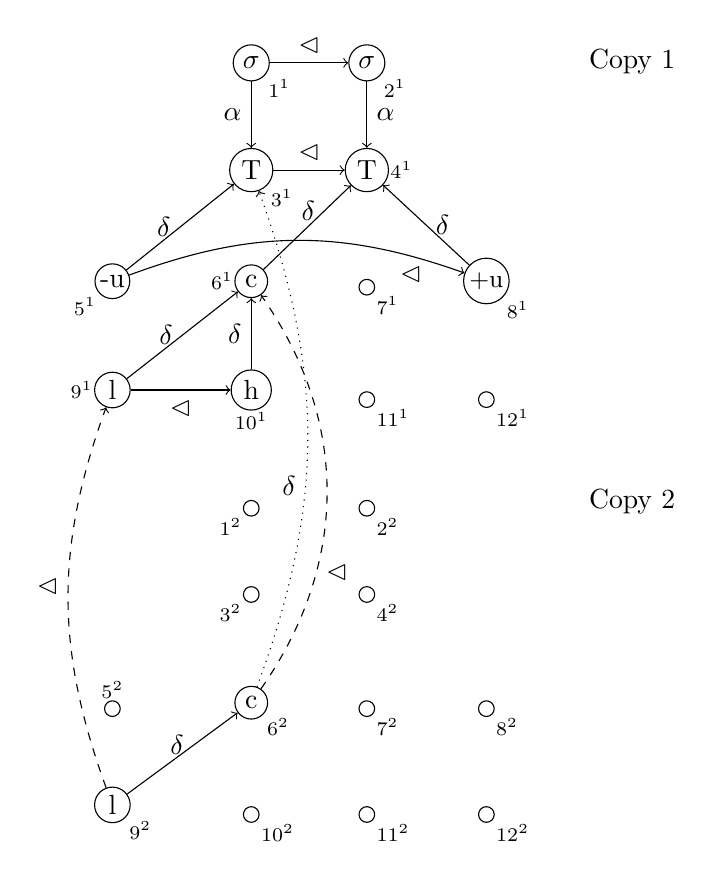
\begin{tikzpicture}[baseline = (x1.base)]
\matrix (m) [matrix of nodes, column sep = 1.5em, row sep = 1.5em]{
& \node[draw,circle, inner sep =2pt,label ={[label distance = -3pt] below right:\scriptsize$1^1$}](x1){$\sigma$};  &  \node[draw,circle, inner sep =2pt,label ={[label distance = -3pt] below right:\scriptsize$2^1$}](x2){$\sigma$}; & & Copy 1 \\
& \node[draw,circle, inner sep =2pt,label ={[label distance = -3pt] below right:\scriptsize$3^1$}](y1){T}; &   \node[draw,circle, inner sep =2pt,label ={[label distance = -3pt] right:\scriptsize$4^1$}](y2){T}; \\
\node[draw,circle, inner sep =1pt,label ={[label distance = -3pt] below left:\scriptsize$5^1$}](z1){-u}; & \node[draw,circle, inner sep =2pt,label ={[label distance = -3pt] left:\scriptsize$6^1$}](z2){c}; &   \node[draw,circle, inner sep =2pt,label ={[label distance = -3pt] below right:\scriptsize$7^1$}](z3){\hspace{1em}}; & \node[draw,circle, inner sep =1pt,label ={[label distance = -3pt] below right:\scriptsize$8^1$}](z4){\se u}; \\
\node[draw,circle, inner sep =2pt,label ={[label distance = -3pt] left:\scriptsize$9^1$}](t1){l}; & \node[draw,circle, inner sep =2pt,label ={[label distance = -3pt] below :\scriptsize$10^1$}](t2){h}; &  \node[draw,circle, inner sep =2pt,label ={[label distance = -3pt] below right:\scriptsize$11^1$}](t3){\hspace{1em}}; & \node[draw,circle, inner sep =2pt,label ={[label distance = -3pt] below right:\scriptsize$12^1$}](t4){\hspace{1em}}; \\
& \node[draw,circle, inner sep =2pt,label ={[label distance = -3pt] below left:\scriptsize$1^2$}](x3){\hspace{1em}}; & \node[draw,circle, inner sep =2pt,label ={[label distance = -3pt] below right:\scriptsize$2^2$}](x4){\hspace{1em}}; & & Copy 2 \\
& \node[draw,circle, inner sep =2pt,label ={[label distance = -3pt] below left:\scriptsize$3^2$}](y3){\hspace{1em}};  & \node[draw,circle, inner sep =2pt,label ={[label distance = -3pt] below right:\scriptsize$4^2$}](y4){\hspace{1em}};\\
\node[draw,circle, inner sep =2pt,label ={[label distance = -3pt] above:\scriptsize$5^2$}](z5){\hspace{1em}};  & \node[draw,circle, inner sep =2pt,label ={[label distance = -3pt] below right:\scriptsize$6^2$}](z6){c}; & \node[draw,circle, inner sep =2pt,label ={[label distance = -3pt] below right:\scriptsize$7^2$}](z7){\hspace{1em}}; & \node[draw,circle, inner sep =2pt,label ={[label distance = -3pt] below right:\scriptsize$8^2$}](z8){\hspace{1em}};   \\
\node[draw,circle, inner sep =2pt,label ={[label distance = -3pt] below right:\scriptsize$9^2$}](t5){l};  & \node[draw,circle, inner sep =2pt,label ={[label distance = -3pt] below right:\scriptsize$10^2$}](t6){\hspace{1em}}; & \node[draw,circle, inner sep =2pt,label ={[label distance = -3pt] below right:\scriptsize$11^2$}](t7){\hspace{1em}}; & \node[draw,circle, inner sep =2pt,label ={[label distance = -3pt] below right:\scriptsize$12^2$}](t8){\hspace{1em}}; \\
};
\draw [->] (x1) -- (y1) node[left, pos=.5]{$\alpha$};
\draw [->](x2) -- (y2) node[right, pos=.5]{$\alpha$};
\draw [->](z1) -- (y1) node[left, pos=.5]{$\delta$};
\draw [->](z2) -- (y2) node[left, pos=.7]{$\delta$};
\draw [<-](z2) -- (t1) node[left, pos=.5]{$\delta$};
\draw [<-](z2) -- (t2) node[left, pos=.5]{$\delta$};
\draw [<-](y2) -- (z4) node[right, pos=.5]{$\delta$};
\draw [->](t5) -- (z6) node [left, pos=.6]{$\delta$};
\path [->,dotted] (z6) edge [bend right = 20] node[left,pos=.4]{$\delta$} (y1);
\draw [->](x1) -- (x2) node[above, pos=.5]{$\vartriangleleft$};
\draw [->](y1) -- (y2) node[above, pos=.5]{$\vartriangleleft$};
\draw [->](t1) -- (t2) node[below, pos=.5]{$\vartriangleleft$};
\path [->](z1) edge [bend left = 20] node[below,pos=.85]{$\vartriangleleft$} (z4);
\path [->,dashed] (z6) edge [bend right = 35] node[right,pos=.3]{$\vartriangleleft$} (z2);
\path [->,dashed] (t5) edge [bend left = 20] node[left,pos=.53]{$\vartriangleleft$} (t1);
\end{tikzpicture}
\end{center}
\section{Transductions between Models}
Throughout the previous sections, we have suggested that a degree of equivalency exists between the Yip and Bao tonal geometries. The goal of this section is to quantify this equivalency by offering transductions between the two models. Here, we prove that it is possible to translate between the two representations using simple (QF) logic. \par
To do so, we will capitalize on structural equivalencies in the models. In the first transduction from Bao's representation to Yip's representation, we observe that the root register node in Yip's tonal geometry is a structural analog of Bao's `T' and `c' nodes; it is the node to which the TBU is associated (`T' in Bao's model), as well as the immediate dominator of terminal tonal nodes (`c' in Bao's model). Additionally, it is a featural analog of Bao's register node (as it is designated as either [+u] or [-u]). The Bao-to-Yip transduction captures this intuition by `fusing' these three nodes, and this fusion is mediated through the only structural position in Bao's model for which relations obtain among all three: the `T' node. \par
The Yip-to-Bao transduction achieves the inverse: it will `explode' Yip's register node into a complex of `r', `T', and `c' nodes. It achieves this by increasing the size of the copy set to three, such that each of the `T', `r', and `c' nodes are defined on the \emph{same structural positions} in their respective copy sets. The relations that unite them (that is, dominance) are defined between copy sets via the identity function ($\ap$).
\subsection{Bao to Yip}
Consider the general transduction $\Gamma^{by}: \mathfrak{M}^{B} \mapsto \mathfrak{M}^{Y}$ from a general Bao model to a general Yip model. The copy set is of size 1.
\begin{equation}
\begin{aligned}
P^{1}_{\sigma}(x)&\myeq P_{\sigma}(x) \\
P^{1}_{+u}(x)&\myeq P_{+u}(x) \\
P^{1}_{-u}(x)&\myeq P_{-u}(x) \\
P^{1}_{h}(x)&\myeq P_{h}(x) \\
P^{1}_{l}(x)&\myeq P_{l}(x) \\
\alpha^{1,1}(x)\ap y&\myeq P_{\sigma}(x) \land P_{r}(y) \land \alpha(x) \ap \delta(y) \\
\delta^{1,1}(x)\ap y&\myeq P_{t}(x)\land P_{r}(y) \land  \delta(\delta(x)) \ap \delta(y)\\
succ^{1,1}(x)\ap y&\myeq succ(x)\ap y \\
\end{aligned}
\end{equation}
Translating from a Bao model to a Yip model does not require the introduction of any featural labels on output nodes which are not already present in the input structure, so the unary relation definitions are preserved through the transduction. Note that this also permits preservation of the successor function into the output. The association and dominance functions, however, must be redefined to reflect the fusion of the `T' and `c' structural positions into a single register node. In the definition of association, the first two conjuncts specify the nodes (syllable and register) which enter into the relation. The third conjunct drives one-to-one association; it does so, however, via the `T' node. The first term ($\alpha(x)$) and second term ($\delta(y)$) point to the \emph{same structural position} in the input, a tautosyllabic `T' node, and are related through identity ($\ap$). This is necessitated by the fact that no direct relation obtains between these nodes in the input structure. `T' in Bao's model, then, is the conduit which connects unrelated input elements, therefore allowing iterative association between syllable and register nodes in a Yip output. \par
Defining the dominance function also leverages the `T' node as the structural position which unites `r' and `t' nodes in the input model. Note that the third conjunct of this definition resembles that of the association definition. The only difference here is that the domain is a $\delta(x)$ function call embedded inside another $\delta(x)$ function call; this isolates the same input `T' node, just from a different structural position (a terminal tonal node). In other words, the `T' node serves as the \emph{placeholder} in the part of the definition which accommodates polysyllabic structures (much like association). This is because `r' is dominated by `T' in the input, and `t' is dominated by the node which `T' dominates (in this case `c'). Register and terminal tonal nodes relate vicariously through `T' in Bao's model, and this is true of no other nodes. \par 
The figure below illustrates the transduction on a disyllabic sequence (the Zhenhai [L.MH] structure).
\begin{center}
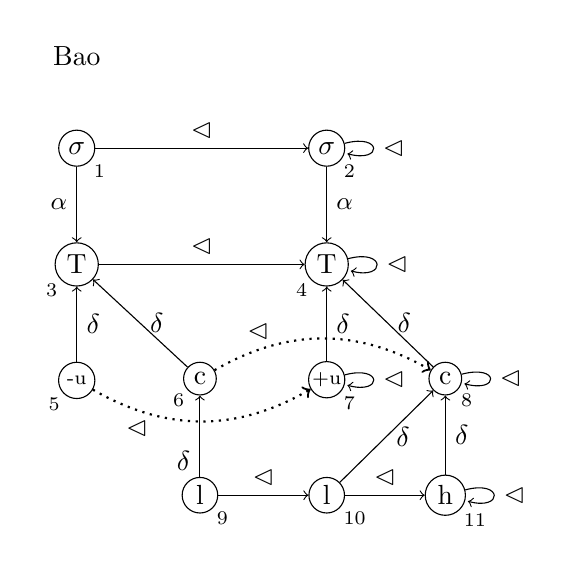
\begin{tikzpicture} [baseline = (y.base)]
\matrix (m) [matrix of nodes, column sep = 1.8em, row sep = 2em]{
Bao \\
\node[draw,circle, inner sep =2pt, label ={[label distance = -3pt] below right:\scriptsize1}](x){$\sigma$}; & &  \node[draw,circle, inner sep =2pt, label ={[label distance = -3pt] below right:\scriptsize2}](x2){$\sigma$};\\
\node[draw,circle, inner sep =2pt, label ={[label distance = -3pt] below left:\scriptsize3}](y){T}; & & \node[draw,circle, inner sep =2pt, label ={[label distance = -3pt] below left:\scriptsize4}](y2){T};& \\
\node[draw,circle, inner sep =2pt, label ={[label distance = -3pt] below left:\scriptsize5}](z){\scriptsize-u};  & \node[draw,circle, inner sep =2pt, label ={[label distance = -3pt] below left:\scriptsize6}](z1){c}; & \node[draw,circle, inner sep =.5pt, label ={[label distance = -3pt] below right:\scriptsize7}](z2){\scriptsize+u}; & \node[draw,circle, inner sep =2pt, label ={[label distance = -3pt] below right:\scriptsize8}](z3){c}; \\
& \node[draw,circle, inner sep =2pt, label ={[label distance = -3pt] below right:\scriptsize9}](t1){l}; & \node[draw,circle, inner sep =2pt, label ={[label distance = -3pt] below right:\scriptsize10}](t2){l}; & \node[draw,circle, inner sep =2pt, label ={[label distance = -3pt] below right:\scriptsize11}](t3){h}; \\
};
\draw [->](x) -- (y) node[left, pos=.5]{\small$\alpha$};
\draw [->](z) -- (y) node[right, pos=.5]{$\delta$};
\draw [->](z1) -- (y) node[right, pos=.5]{$\delta$};
\draw [->](x2) -- (y2) node[right, pos=.5]{\small$\alpha$};
\draw [->](z2) -- (y2) node[right, pos=.5]{$\delta$};
\draw [->](t1) -- (z1) node[left, pos=.2]{$\delta$};
\draw [->](t2) -- (z3) node[right, pos=.5]{$\delta$};
\draw [->](t3) -- (z3) node[right, pos=.5]{$\delta$};
\draw [->](z3) -- (y2) node[right, pos=.5]{$\delta$};
\draw [->](x) -- (x2) node[above, pos=.5]{$\vartriangleleft$};
\draw [->](t1) -- (t2) node[above, pos=.5]{$\vartriangleleft$};
\draw [->](t2) -- (t3) node[above, pos=.5]{$\vartriangleleft$};
\draw [->](y) -- (y2) node[above, pos=.5]{$\vartriangleleft$};
\path (x2) edge [loop right] node{$\vartriangleleft$} (x2);
\path (y2) edge [loop right] node{$\vartriangleleft$} (y2);
\path (z3) edge [loop right] node{$\vartriangleleft$} (z3);
\path (z2) edge [loop right] node{$\vartriangleleft$} (z2);
\path (t3) edge [loop right] node{$\vartriangleleft$} (t3);
\path [thick, dotted, ->] (z) edge [bend right=30] node[below,pos=.2]{$\vartriangleleft$} (z2);
\path [thick, dotted, ->] (z1) edge [bend left=30] node[above,pos=.2]{$\vartriangleleft$} (z3);
\end{tikzpicture}
\hspace{.3cm}
$\rightarrow$
\hspace{.5cm}
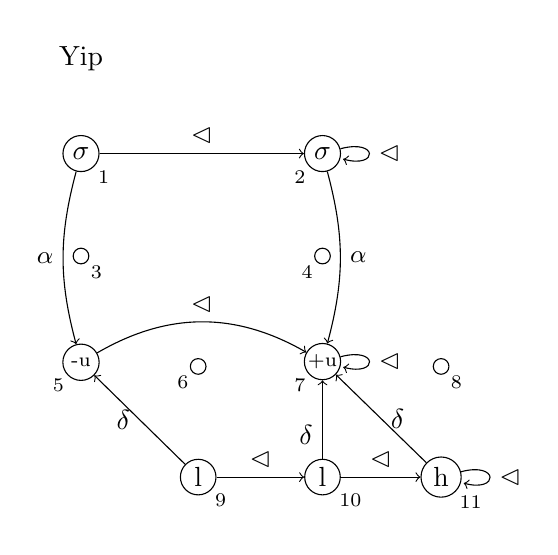
\begin{tikzpicture} [baseline = (y.base)]
\matrix (m) [matrix of nodes, column sep = 1.8em, row sep = 2em]{
Yip \\
\node[draw,circle, inner sep =2pt, label ={[label distance = -3pt] below right:\scriptsize1}](x){$\sigma$}; & &  \node[draw,circle, inner sep =2pt, label ={[label distance = -3pt] below left:\scriptsize2}](x2){$\sigma$};\\
\node[draw,circle, inner sep =2pt, label ={[label distance = -3pt] below right:\scriptsize3}](y){\hspace{1em}}; & & \node[draw,circle, inner sep =2pt, label ={[label distance = -3pt] below left:\scriptsize4}](y2){\hspace{1em}};& \\
\node[draw,circle, inner sep =2pt, label ={[label distance = -3pt] below left:\scriptsize5}](z){\scriptsize-u};  & \node[draw,circle, inner sep =2pt, label ={[label distance = -3pt] below left:\scriptsize6}](z1){\hspace{1em}}; & \node[draw,circle, inner sep =.5pt, label ={[label distance = -3pt] below left:\scriptsize7}](z2){\scriptsize+u}; & \node[draw,circle, inner sep =2pt, label ={[label distance = -3pt] below right:\scriptsize8}](z3){\hspace{1em}}; \\
& \node[draw,circle, inner sep =2pt, label ={[label distance = -3pt] below right:\scriptsize9}](t1){l}; & \node[draw,circle, inner sep =2pt, label ={[label distance = -3pt] below right:\scriptsize10}](t2){l}; & \node[draw,circle, inner sep =2pt, label ={[label distance = -3pt] below right:\scriptsize11}](t3){h}; \\
};
\path [->] (x) edge[bend right=15] node[left, pos=.5]{\small$\alpha$}(z);
\path [->] (x2) edge[bend left=15] node[right,pos=.5]{\small$\alpha$}(z2);
\draw [->](x) -- (x2) node[above, pos=.5]{$\vartriangleleft$};
\draw [->](t1) -- (t2) node[above, pos=.5]{$\vartriangleleft$};
\draw [->](t2) -- (t3) node[above, pos=.5]{$\vartriangleleft$};
\draw [->](t2) -- (z2) node[left, pos=.3]{$\delta$};
\draw [->](t3) -- (z2) node[right, pos=.5]{$\delta$};
\draw [->](t1) -- (z) node[left, pos=.5]{$\delta$};
\path (x2) edge [loop right] node{$\vartriangleleft$} (x2);
\path (z2) edge [loop right] node{$\vartriangleleft$} (z2);
\path (t3) edge [loop right] node{$\vartriangleleft$} (t3);
\path [ ->] (z) edge [bend left=30] node[above,pos=.5]{$\vartriangleleft$} (z2);
\end{tikzpicture}
\end{center}
\subsection{Yip to Bao}
Consider the general transduction $\Gamma^{yb}: \mathfrak{M}^{Y}\mapsto \mathfrak{M}^{B}$ from a general Yip model to a general Bao model. The copy set is of size 3.
\begin{equation}
\begin{aligned}
\sigma&\text{/`T'} & \text{regis}&\text{ter} & \text{`c'}&\text{/`t'} \\
P^{1}_{\sigma}(x) &\myeq P_{\sigma}(x) & P^{2}_{\sigma}(x) &\myeq \mathtt{F} & P^{3}_{\sigma}(x) &\myeq \mathtt{F} \\
P^{1}_{T}(x) &\myeq P_{r}(x) & P^{2}_{T}(x) &\myeq \mathtt{F} & P^{3}_{T}(x) &\myeq \mathtt{F} \\
P^{1}_{+u}(x) &\myeq \mathtt{F}  & P^{2}_{+u}(x) &\myeq P_{r}(x) & P^{3}_{+u}(x) &\myeq \mathtt{F} \\ 
P^{1}_{-u}(x) &\myeq \mathtt{F}  & P^{2}_{-u}(x) &\myeq P_{r}(x) & P^{3}_{-u}(x) &\myeq \mathtt{F} \\ 
P^{1}_{c}(x) &\myeq \mathtt{F}  & P^{2}_{c}(x) &\myeq \mathtt{F} & P^{3}_{c}(x) &\myeq P_{r}(x)  \\ 
P^{1}_{h}(x) &\myeq \mathtt{F}  & P^{2}_{h}(x) &\myeq \mathtt{F} & P^{3}_{h}(x) &\myeq P_{t}(x)  \\
P^{1}_{l}(x) &\myeq \mathtt{F}  & P^{2}_{l}(x) &\myeq \mathtt{F} & P^{3}_{l}(x) &\myeq P_{t}(x)  \\
\alpha^{1,1}(x)\ap y &\myeq \alpha(x)\ap y & \alpha^{1,2}(x)\ap y &\myeq \mathtt{F} & \alpha^{1,3}(x)\ap y &\myeq \mathtt{F} \\
\alpha^{2,1}(x)\ap y &\myeq \mathtt{F} & \alpha^{2,2}(x)\ap y &\myeq \mathtt{F} & \alpha^{2,3}(x)\ap y &\myeq \mathtt{F} \\
\alpha^{3,1}(x)\ap y &\myeq \mathtt{F} & \alpha^{3,2}(x)\ap y &\myeq \mathtt{F} & \alpha^{3,3}(x)\ap y &\myeq \mathtt{F} \\
\delta^{1,1}(x)\ap y &\myeq \mathtt{F} & \delta^{1,2}(x)\ap y &\myeq \mathtt{F} & \delta^{1,3}(x)\ap y &\myeq \mathtt{F} \\
\delta^{2,1}(x)\ap y &\myeq P_{r}(x)\land P_{r}(y)\land x\ap y & \delta^{2,2}(x)\ap y &\myeq \mathtt{F} & \delta^{3,3}(x)\ap y &\myeq \mathtt{F} \\
\delta^{3,1}(x)\ap y &\myeq P_{r}(x)\land P_{r}(y)\land x\ap y & \delta^{2,2}(x)\ap y &\myeq \mathtt{F} & \delta^{3,3}(x)\ap y &\myeq \delta(x)\ap y \\
succ^{1,1}(x)\ap y &\myeq succ(x)\ap y & succ^{1,2}(x)\ap y &\myeq \mathtt{F} & succ^{1,3}(x)\ap y &\myeq \mathtt{F} \\
succ^{2,1}(x)\ap y &\myeq \mathtt{F} & succ^{2,2}(x)\ap y &\myeq succ(x)\ap y & succ^{2,3}(x)\ap y &\myeq \mathtt{F} \\
succ^{3,1}(x)\ap y &\myeq \mathtt{F}  & succ^{3,2}(x)\ap y &\myeq \mathtt{F} & succ^{3,3}(x)\ap y &\myeq succ(x)\ap y \\
\end{aligned}
\end{equation}
This general transduction $\Gamma^{yb}$ seizes on the intuition that the `r' node in the Yip model is the structural equivalent of both the Bao `c' and Bao `T' node, and is the featural equivalent of Bao's register node. To translate from Yip's representation to Bao's, we `explode' the register node into independent register, `T' and `c' nodes. This is achieved across three copy sets, one for each `instantiation' of Yip's register node. The figure below schematizes the transduction, where syllable and `T' nodes populate the first copy set, the register node occupies the second copy set, and the `c' and terminal tonal nodes are defined on the third copy set. Successor relations are omitted for clarity.
\begin{center}
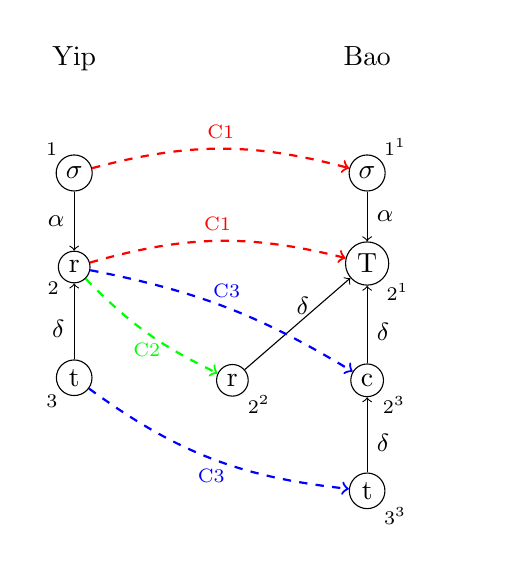
\begin{tikzpicture} [baseline = (x.base)]
\matrix (m) [matrix of nodes, column sep = 2em, row sep = 1.8em]{
Yip & & & Bao \\
\node[draw,circle, inner sep =2pt, label ={[label distance = -3pt] above left:\scriptsize1}](x){$\sigma$}; & & &  \node[draw,circle, inner sep =2pt, label ={[label distance = -3pt] above right:\scriptsize$1^1$}](x2){$\sigma$};\\
\node[draw,circle, inner sep =2pt, label ={[label distance = -3pt] below left:\scriptsize2}](y){r}; & & & \node[draw,circle, inner sep =2pt, label ={[label distance = -3pt] below right:\scriptsize$2^1$}](y2){T};& \\
\node[draw,circle, inner sep =2pt, label ={[label distance = -3pt] below left:\scriptsize3}](z){t}; & & \node[draw,circle, inner sep =2pt, label ={[label distance = -3pt] below right:\scriptsize$2^2$}](z2){r};& \node[draw,circle, inner sep =2pt, label ={[label distance = -3pt] below right:\scriptsize$2^3$}](z3){c};& \\
& & & \node[draw,circle, inner sep =2pt, label ={[label distance = -3pt] below right:\scriptsize$3^3$}](t){t};& \\
};
\draw [->] (x) -- (y) node[left, pos=.5]{\small$\alpha$};
\draw [->] (x2) -- (y2) node[right, pos=.5]{\small$\alpha$};
\draw [->] (z) -- (y) node[left, pos=.4]{\small$\delta$};
\draw [->] (z2) -- (y2) node[left, pos=.7]{\small$\delta$};
\draw [->] (z3) -- (y2) node[right, pos=.4]{\small$\delta$};
\draw [->] (t) -- (z3) node[right, pos=.4]{\small$\delta$};
\path [color = red, thick, dashed, ->] (x) edge[bend left=15] node[above]{\scriptsize C1} (x2);
\path [color = red, thick, dashed, ->] (y) edge[bend left=15] node[above]{\scriptsize C1} (y2);
\path [color = green, thick, dashed, ->] (y) edge[bend right=10] node[below]{\scriptsize C2} (z2);
\path [color = blue, thick, dashed, ->] (y) edge[bend left=10] node[above]{\scriptsize C3} (z3);
\path [color = blue, thick, dashed, ->] (z) edge[bend right=15] node[below]{\scriptsize C3} (t);
\end{tikzpicture}
\end{center} \par
Let us examine the transduction in more detail. The first copy set houses the syllable nodes and the register-`T' equivalency, that is, the node which is the codomain of $\alpha(x)\ap y$. Unary relations on syllable and root `T' nodes are specified for the first copy set (with the latter defined in terms of input $P_{r}(x)$), and are set to False for the second and third. Similarly, the input association function is preserved on the first copy set; this ensures that TBU-root association proceeds one-to-one, provided that the Yip input satisfies Axioms I-III. Ordering on these elements is preserved. \par
In the second copy set, the unary relation definition on register nodes $P^{2}_{r}(x)$ underlies the featural equivalence of register nodes between both models. Having defined register nodes, we must establish a dominance relation such that the function $\delta(x)\ap y$ comprises a domain of register nodes from copy set two and a codomain of `T' nodes from copy set one (which, recall, occupy the structural position of register nodes). This work is done by the first two conjuncts, which select register nodes from copy sets 2 and 1. Since our goal is to isolate r-T pairs which share a structural position (thus keeping dominance within syllables and not across them), we define the function from the second copy set to the first with a third conjunct, relating these nodes via the identity function. Here, we take the identity function (x$\ap$y) to select a unique element position within a copy set. The effect is that register nodes are dominated by tautosyllabic `T' nodes \emph{only}. The dominance function $\delta^{2,1}(x)\ap y$ takes a unique register node from copy set two and outputs the identical structural position in copy set 1 (a `T' node). Again, the successor function is preserved from the input.\par
The third copy set contains tonal `t' elements and the register-`c' equivalency, that is, the structural position that serves as the immediate dominator of terminal tonal nodes. The unary relation $P^{3}_{c}(x)$ conflates output `c' and input register ($P_{r}(x)$) nodes. Domination of terminal `t' nodes, then, is preserved from the input structure (def. $\delta^{3,3}(x)\ap y$). Contour `c' node (in copy set three) domination under the root `T' node (in copy set one) proceeds as it did with the register node (register and `c' nodes are sisters in Bao's model); the binary dominance function $\delta^{3,1}(x)\ap y$ is defined as that from copy set 2 to copy set 1: unary predicates which select register nodes, followed by positional identity between copy sets. Ordering is also preserved from the input model. \par
The successor function is defined for elements \emph{within} copy sets only. This ensures that linear order obtains for elements on the same tier, and not across tiers, as is our desired effect. The definition of the successor function is preserved from the input, imposing order on intra-tier elements within their respective copy sets: syllable nodes and `T' nodes in the first copy set, register nodes in the second copy set, and `c' and terminal tonal nodes in the third copy set. \par
The figure below illustrates the output of the transduction on a disyllabic sequence (the Zhenhai [L.MH] structure).
\begin{center}
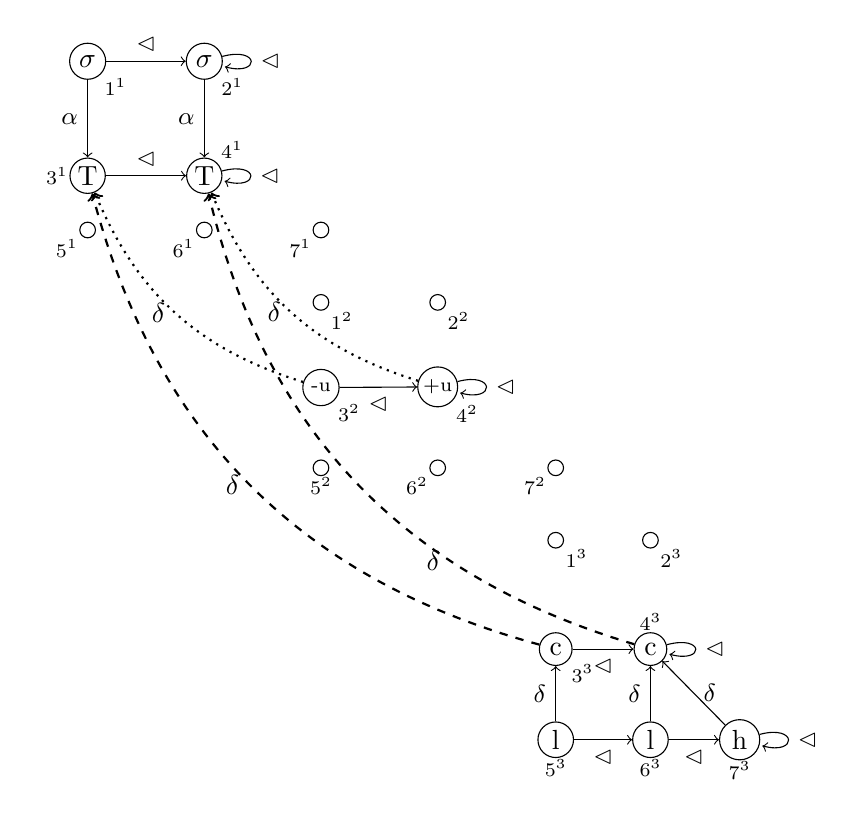
\begin{tikzpicture} [baseline = (x.base)]
\matrix (m) [matrix of nodes, column sep = 1em, row sep = 1em]{
\node[draw,circle, inner sep =2pt, label ={[label distance = -3pt] below right:\scriptsize$1^1$}](x){$\sigma$}; &   \node[draw,circle, inner sep =2pt, label ={[label distance = -3pt] below right:\scriptsize$2^1$}](x2){$\sigma$}; \\
\node[draw,circle, inner sep =1pt, label ={[label distance = -3pt] left:\scriptsize$3^1$}](y){T}; &  \node[draw,circle, inner sep =1pt, label ={[label distance = -3pt] above right:\scriptsize$4^1$}](y2){T}; \\
\node[draw,circle, inner sep =2pt, label ={[label distance = -3pt] below left:\scriptsize$5^1$}](t){\hspace{1em}};  & \node[draw,circle, inner sep =2pt, label ={[label distance = -3pt] below left:\scriptsize$6^1$}](t2){\hspace{1em}}; & \node[draw,circle, inner sep =2pt, label ={[label distance = -3pt] below left:\scriptsize$7^1$}](t3){\hspace{1em}}; \\
& &  \node[draw,circle, inner sep =2pt, label ={[label distance = -3pt] below right:\scriptsize$1^2$}](xx){\hspace{1em}}; &   \node[draw,circle, inner sep =2pt, label ={[label distance = -3pt] below right:\scriptsize$2^2$}](xx2){\hspace{1em}};\\
& &  \node[draw,circle, inner sep =2pt, label ={[label distance = -3pt] below right:\scriptsize$3^2$}](yy){\scriptsize-u}; &  \node[draw,circle, inner sep =1pt, label ={[label distance = -3pt] below right:\scriptsize$4^2$}](yy2){\scriptsize+u}; \\
& &  \node[draw,circle, inner sep =2pt, label ={[label distance = -3pt] below:\scriptsize$5^2$}](tt){\hspace{1em}};  & \node[draw,circle, inner sep =2pt, label ={[label distance = -3pt] below left:\scriptsize$6^2$}](tt2){\hspace{1em}}; & \node[draw,circle, inner sep =2pt, label ={[label distance = -3pt] below left:\scriptsize$7^2$}](tt3){\hspace{1em}}; \\
& & & & \node[draw,circle, inner sep =2pt, label ={[label distance = -3pt] below right:\scriptsize$1^3$}](xxx){\hspace{1em}}; &   \node[draw,circle, inner sep =2pt, label ={[label distance = -3pt] below right:\scriptsize$2^3$}](xxx2){\hspace{1em}};\\
& & & & \node[draw,circle, inner sep =2pt, label ={[label distance = -3pt] below right:\scriptsize$3^3$}](yyy){c}; &  \node[draw,circle, inner sep =2pt, label ={[label distance = -3pt] above:\scriptsize$4^3$}](yyy2){c}; \\
& & & & \node[draw,circle, inner sep =2pt, label ={[label distance = -3pt] below:\scriptsize$5^3$}](ttt){l};  & \node[draw,circle, inner sep =2pt, label ={[label distance = -3pt] below:\scriptsize$6^3$}](ttt2){l}; & \node[draw,circle, inner sep =2pt, label ={[label distance = -3pt] below:\scriptsize$7^3$}](ttt3){h}; \\
};
\draw[->] (x) -- (y) node[left, pos=.5]{\small$\alpha$};
\draw[->] (x2) -- (y2) node[left, pos=.5]{\small$\alpha$};
\path [thick, dotted,->] (yy) edge[bend left=25] node[left]{$\delta$} (y);
\path [thick, dotted,->] (yy2) edge[bend left = 25] node[left]{$\delta$} (y2);
\path [thick, dashed,->] (yyy) edge[bend left=30] node[left]{$\delta$} (y);
\path [thick, dashed,->] (yyy2) edge[bend left = 30] node[left,pos=.3]{$\delta$} (y2);
\path (x2) edge [loop right] node{\small$\vartriangleleft$} (x2);
\path (y2) edge [loop right] node{\small$\vartriangleleft$} (y2);
\path (yy2) edge [loop right] node{\small$\vartriangleleft$} (yy2);
\path (yyy2) edge [loop right] node{\small$\vartriangleleft$} (yyy2);
\path (ttt3) edge [loop right] node{\small$\vartriangleleft$} (ttt3);
\draw[->] (ttt) -- (yyy) node[left, pos=.5]{\small$\delta$};
\draw[->] (ttt2) -- (yyy2) node[left, pos=.5]{\small$\delta$};
\draw[->] (ttt3) -- (yyy2) node[right, pos=.5]{\small$\delta$};
\draw[->] (x) -- (x2) node[above, pos=.5]{\small$\vartriangleleft$};
\draw[->] (y) -- (y2) node[above, pos=.5]{\small$\vartriangleleft$};
\draw[->] (yy) -- (yy2) node[below, pos=.5]{\small$\vartriangleleft$};
\draw[->] (yyy) -- (yyy2) node[below, pos=.5]{\small$\vartriangleleft$};
\draw[->] (ttt) -- (ttt2) node[below, pos=.5]{\small$\vartriangleleft$};
\draw[->] (ttt2) -- (ttt3) node[below, pos=.5]{\small$\vartriangleleft$};
\end{tikzpicture}
\end{center}
\subsection{Summary}
In this section, we have shown that, at some level, the Yip and Bao tonal geometries are notationally equivalent. We defined transductions between both models using a logic of relatively low complexity (Quantifier-Free First-Order), capitalizing on the intuition that Yip's model condenses three of Bao's structural nodes into a single node (r-T-c $\rightarrow$ r), and that Bao's model expands one of Yip's structural nodes into three distinct ones (r $\rightarrow$ r-T-c).  
\section{Transception: A Transduction \emph{within} a Transduction}
So far, we have illustrated the mutual QF-interpretability between Yip and Bao models. Now, we perform transductions on models of a specific process that is argued to be possible in Bao's representation but \emph{impossible} using Yip's tonal geometry: Zhenhai contour shift. Specifically, we introduce a simplified version of the transduction in Section 2 (Zhenhai contour shift in Bao's model). We then apply $\Gamma^{by}$ to the input of the transduction \emph{and its output} and examine the results. This is schematized below:
\begin{center}
\begin{tabular}{ccccc}
& & {\small$\tau^{B}_{zh}$} \\
& $\mathcal{M}^{B}_{I}$ & {\Large$\mapsto$} & $\mathcal{M}^{B}_{O}$ \\
\hspace{1em} \\
{\small$\Gamma^{by}$} & {\Large$\downmapsto$} & & {\Large$\downmapsto$} & {\small$\Gamma^{by}$} \\ 
\hspace{1em} \\
& $\mathcal{M}^{Y}_{I}$ & {\Large$\mapsto$} & $\mathcal{M}^{Y}_{O}$ \\
& & {\small\underline{$\tau^{Y}_{zh}$(QF?)}} \\
\end{tabular}
\end{center}
The question that concerns us here is: modeling the Zhenhai pattern, if a transduction ($\Gamma^{by}$) from a Bao input model to a Yip input model is QF, and if this same transduction is applied to a Bao output model (itself the result of a QF transduction ($\tau^{B}_{zh}$) on the Bao input model) to yield a Yip output model, would a transduction directly from a Yip input to a Yip output (the underlined transduction in the figure above) yield the same structure while \emph{also} being QF? And if so, what does this say about earlier claims that such processes cannot be modeled in Yip's representation, or any process for that matter? \par
This section addresses these questions as follows. First, we define a model over a Zhenhai input in Bao's representation ($\mathcal{M}^{B}_{I}$). Then we perform $\Gamma^{by}$ on this model to yield a corresponding Zhenhai input in Yip ($\mathcal{M}^{Y}_{I}$). The simplified QF I/O transduction modeling contour shift ($\tau^{B}_{zh}$) is then introduced and applied to the Bao input. This transduction's output is then fed into $\Gamma^{by}$ to produce a post-contour shift Yip output model. We then pause to compare the outputs, and consider what a contour shift transduction directly from a Yip input to Yip output might entail.
\subsection{Bao Input Model: $\mathcal{M}^{B}_{I}$}
Let $\mathcal{M}^{B}_{I}$ be a model of a Zhenhai input structure in Bao's representation: a disyllabic form [LM.HL].
\begin{equation}
\begin{aligned}
\mathcal{M}^{B}_{I} \myeq \langle \mathcal{D}; &P_{\sigma}, P_{T}, P_{+u}, P_{-u}, P_{h}, P_{l}, P_{c}; \\
\alpha(x)\ap y, &\delta(x)\ap y, succ(x)\ap y \rangle \\
\mathcal{D} &= \{1, 2, 3, 4, 5, 6, 7, 8, 9, 10, 11, 12\}  \\
P_{\sigma} &= \{1, 2\} & P_{T} &= \{3, 4\} \\
P_{+u} &= \{7\} & P_{-u} &= \{5\} \\
P_{h} &= \{10, 11\} & P_{l} &= \{9, 12\} \\ 
P_{c} &= \{6, 8\}& \alpha(x)\ap y &= \begin{cases} 3 & x=1 \\ 4 & x=2 \end{cases}  \\
 \delta(x)\ap y &= \begin{cases} 3 & x\in\{5,6\} \\ 4 & x\in \{7,8\} \\ 6 & x\in\{9,10\} \\ 8 & x\in\{11,12\} \end{cases} &
succ(x)\ap y &= \begin{cases} 2 & x\in \{1,2\} \\ 4 & x\in \{3,4\} \\ 7 & x\in\{5,7\} \\ 8 & x\in\{6,8\} \\ 10 & x=9 \\ 11 & x=10 \\ 12 & x\in\{11,12\} \end{cases} \\
\end{aligned}
\end{equation}
The graphical representation of $\mathcal{M}^{B}_{I}$ is thus:
\begin{center}
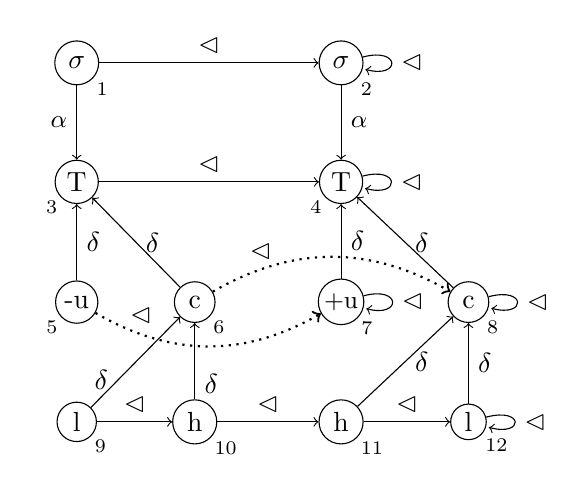
\begin{tikzpicture} [baseline = (x.base)]
\matrix (m) [matrix of nodes, column sep = 2em, row sep = 2em]{
\node[draw,circle, inner sep =3pt, label ={[label distance = -3pt] below right:\scriptsize1}](x){$\sigma$}; & &  \node[draw,circle, inner sep =3pt, label ={[label distance = -3pt] below right:\scriptsize2}](x2){$\sigma$};\\
\node[draw,circle, inner sep =2pt, label ={[label distance = -3pt] below left:\scriptsize3}](y){T}; & & \node[draw,circle, inner sep =2pt, label ={[label distance = -3pt] below left:\scriptsize4}](y2){T};& \\
\node[draw,circle, inner sep =2pt, label ={[label distance = -3pt] below left:\scriptsize5}](z){-u};  & \node[draw,circle, inner sep =3pt, label ={[label distance = -3pt] below right:\scriptsize6}](z1){c}; & \node[draw,circle, inner sep =1pt, label ={[label distance = -3pt] below right:\scriptsize7}](z2){\se u}; & \node[draw,circle, inner sep =3pt, label ={[label distance = -3pt] below right:\scriptsize8}](z3){c}; \\
\node[draw,circle, inner sep =2.5pt, label ={[label distance = -3pt] below right:\scriptsize9}](t){l};& \node[draw,circle, inner sep =2.5pt, label ={[label distance = -3pt] below right:\scriptsize10}](t1){h}; & \node[draw,circle, inner sep =2.5pt, label ={[label distance = -3pt] below right:\scriptsize11}](t2){h}; & \node[draw,circle, inner sep =2pt, label ={[label distance = -3pt] below right:\scriptsize12}](t3){l}; \\
};
\draw [->](x) -- (y) node[left, pos=.5]{\small$\alpha$};
\draw [->](z) -- (y) node[right, pos=.5]{$\delta$};
\draw [->](z1) -- (y) node[right, pos=.5]{$\delta$};
\draw [->](x2) -- (y2) node[right, pos=.5]{\small$\alpha$};
\draw [->](z2) -- (y2) node[right, pos=.5]{$\delta$};
\draw [->](t1) -- (z1) node[right, pos=.2]{$\delta$};
\draw [->](t) -- (z1) node[left, pos=.3]{$\delta$};
\draw [->](t2) -- (z3) node[right, pos=.5]{$\delta$};
\draw [->](t3) -- (z3) node[right, pos=.5]{$\delta$};
\draw [->](z3) -- (y2) node[right, pos=.5]{$\delta$};
\draw [->](x) -- (x2) node[above, pos=.5]{$\vartriangleleft$};
\draw [->](t) -- (t1) node[above, pos=.5]{$\vartriangleleft$};
\draw [->](t1) -- (t2) node[above, pos=.5]{$\vartriangleleft$};
\draw [->](t2) -- (t3) node[above, pos=.5]{$\vartriangleleft$};
\draw [->](y) -- (y2) node[above, pos=.5]{$\vartriangleleft$};
\path (x2) edge [loop right] node{$\vartriangleleft$} (x2);
\path (y2) edge [loop right] node{$\vartriangleleft$} (y2);
\path (z3) edge [loop right] node{$\vartriangleleft$} (z3);
\path (z2) edge [loop right] node{$\vartriangleleft$} (z2);
\path (t3) edge [loop right] node{$\vartriangleleft$} (t3);
\path [thick, dotted, ->] (z) edge [bend right=30] node[above,pos=.2]{$\vartriangleleft$} (z2);
\path [thick, dotted, ->] (z1) edge [bend left=30] node[above,pos=.2]{$\vartriangleleft$} (z3);
\end{tikzpicture}
\end{center}
\subsection{General Transduction on Bao Input: $\Gamma^{by}: \mathcal{M}^{B}_{I} \mapsto \mathcal{M}^{Y}_{I}$}
We now perform the QF general transduction $\Gamma^{by}$ on the Bao input model $\mathcal{M}^{B}_{I}$ to yield a model of the corresponding Yip representation model ($\mathcal{M}^{Y}_{I}$). Recall the definition of this transduction:
\begin{equation}
\begin{aligned}
P^{1}_{\sigma}(x)&\myeq P_{\sigma}(x) \\
P^{1}_{+u}(x)&\myeq P_{+u}(x) \\
P^{1}_{-u}(x)&\myeq P_{-u}(x) & \alpha^{1,1}(x)\ap y&\myeq P_{\sigma}(x) \land P_{r}(y) \land \alpha(x) \ap \delta(y) \\
P^{1}_{h}(x)&\myeq P_{h}(x) & \delta^{1,1}(x)\ap y&\myeq P_{t}(x)\land P_{r}(y) \land  \delta(\delta(x)) \ap \delta(y) \\
P^{1}_{l}(x)&\myeq P_{l}(x) & succ^{1,1}(x)\ap y&\myeq succ(x)\ap y \\
\end{aligned}
\end{equation}
The result of this transduction is a model of the Zhenhai form [LM.HL] in Yip's representation; `T', `c' and register nodes have been fused into a single register node.
\begin{center}
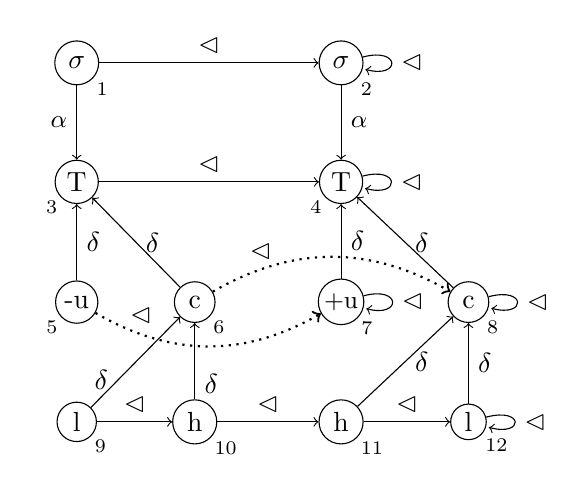
\begin{tikzpicture} [baseline = (y.base)]
\matrix (m) [matrix of nodes, column sep = 2em, row sep = 2em]{
\node[draw,circle, inner sep =3pt, label ={[label distance = -3pt] below right:\scriptsize1}](x){$\sigma$}; & &  \node[draw,circle, inner sep =3pt, label ={[label distance = -3pt] below right:\scriptsize2}](x2){$\sigma$};\\
\node[draw,circle, inner sep =2pt, label ={[label distance = -3pt] below left:\scriptsize3}](y){T}; & & \node[draw,circle, inner sep =2pt, label ={[label distance = -3pt] below left:\scriptsize4}](y2){T};& \\
\node[draw,circle, inner sep =2pt, label ={[label distance = -3pt] below left:\scriptsize5}](z){-u};  & \node[draw,circle, inner sep =3pt, label ={[label distance = -3pt] below right:\scriptsize6}](z1){c}; & \node[draw,circle, inner sep =1pt, label ={[label distance = -3pt] below right:\scriptsize7}](z2){\se u}; & \node[draw,circle, inner sep =3pt, label ={[label distance = -3pt] below right:\scriptsize8}](z3){c}; \\
\node[draw,circle, inner sep =2.5pt, label ={[label distance = -3pt] below right:\scriptsize9}](t){l};& \node[draw,circle, inner sep =2.5pt, label ={[label distance = -3pt] below right:\scriptsize10}](t1){h}; & \node[draw,circle, inner sep =2.5pt, label ={[label distance = -3pt] below right:\scriptsize11}](t2){h}; & \node[draw,circle, inner sep =2pt, label ={[label distance = -3pt] below right:\scriptsize12}](t3){l}; \\
};
\draw [->](x) -- (y) node[left, pos=.5]{\small$\alpha$};
\draw [->](z) -- (y) node[right, pos=.5]{$\delta$};
\draw [->](z1) -- (y) node[right, pos=.5]{$\delta$};
\draw [->](x2) -- (y2) node[right, pos=.5]{\small$\alpha$};
\draw [->](z2) -- (y2) node[right, pos=.5]{$\delta$};
\draw [->](t1) -- (z1) node[right, pos=.2]{$\delta$};
\draw [->](t) -- (z1) node[left, pos=.3]{$\delta$};
\draw [->](t2) -- (z3) node[right, pos=.5]{$\delta$};
\draw [->](t3) -- (z3) node[right, pos=.5]{$\delta$};
\draw [->](z3) -- (y2) node[right, pos=.5]{$\delta$};
\draw [->](x) -- (x2) node[above, pos=.5]{$\vartriangleleft$};
\draw [->](t) -- (t1) node[above, pos=.5]{$\vartriangleleft$};
\draw [->](t1) -- (t2) node[above, pos=.5]{$\vartriangleleft$};
\draw [->](t2) -- (t3) node[above, pos=.5]{$\vartriangleleft$};
\draw [->](y) -- (y2) node[above, pos=.5]{$\vartriangleleft$};
\path (x2) edge [loop right] node{$\vartriangleleft$} (x2);
\path (y2) edge [loop right] node{$\vartriangleleft$} (y2);
\path (z3) edge [loop right] node{$\vartriangleleft$} (z3);
\path (z2) edge [loop right] node{$\vartriangleleft$} (z2);
\path (t3) edge [loop right] node{$\vartriangleleft$} (t3);
\path [thick, dotted, ->] (z) edge [bend right=30] node[above,pos=.2]{$\vartriangleleft$} (z2);
\path [thick, dotted, ->] (z1) edge [bend left=30] node[above,pos=.2]{$\vartriangleleft$} (z3);
\end{tikzpicture}
\hspace{1cm}
$\mapsto$
\hspace{1cm}
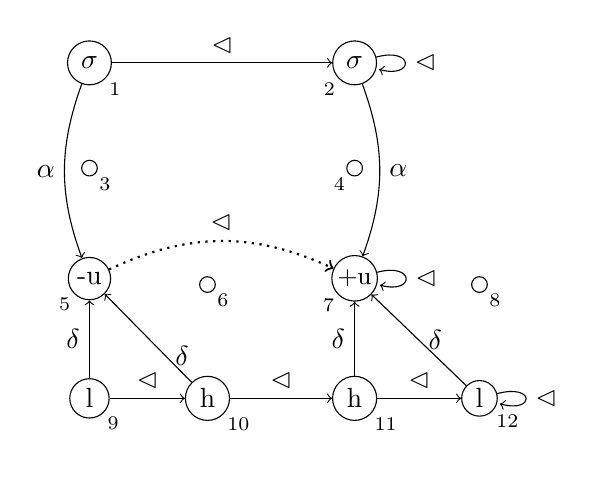
\begin{tikzpicture} [baseline = (y.base)]
\matrix (m) [matrix of nodes, column sep = 2em, row sep = 2em]{
\node[draw,circle, inner sep =3pt, label ={[label distance = -3pt] below right:\scriptsize1}](x){$\sigma$}; & &  \node[draw,circle, inner sep =3pt, label ={[label distance = -3pt] below left:\scriptsize2}](x2){$\sigma$};\\
\node[draw,circle, inner sep =2pt, label ={[label distance = -3pt] below right:\scriptsize3}](y){\hspace{1em}}; & & \node[draw,circle, inner sep =2pt, label ={[label distance = -3pt] below left:\scriptsize4}](y2){\hspace{1em}};& \\
\node[draw,circle, inner sep =2pt, label ={[label distance = -3pt] below left:\scriptsize5}](z){-u};  & \node[draw,circle, inner sep =2pt, label ={[label distance = -3pt] below right:\scriptsize6}](z1){\hspace{1em}}; & \node[draw,circle, inner sep =1pt, label ={[label distance = -3pt] below left:\scriptsize7}](z2){\se u}; & \node[draw,circle, inner sep =2pt, label ={[label distance = -3pt] below right:\scriptsize8}](z3){\hspace{1em}}; \\
\node[draw,circle, inner sep =2.5pt, label ={[label distance = -3pt] below right:\scriptsize9}](t){l};& \node[draw,circle, inner sep =2.5pt, label ={[label distance = -3pt] below right:\scriptsize10}](t1){h}; & \node[draw,circle, inner sep =2.5pt, label ={[label distance = -3pt] below right:\scriptsize11}](t2){h}; & \node[draw,circle, inner sep =2pt, label ={[label distance = -3pt] below right:\scriptsize12}](t3){l}; \\
};
\draw [->](x) -- (x2) node[above, pos=.5]{$\vartriangleleft$};
\draw [->](t) -- (t1) node[above, pos=.5]{$\vartriangleleft$};
\draw [->](t1) -- (t2) node[above, pos=.5]{$\vartriangleleft$};
\draw [->](t2) -- (t3) node[above, pos=.5]{$\vartriangleleft$};
\draw [->](t) -- (z) node[left, pos=.5]{$\delta$};
\draw [->](t1) -- (z) node[right, pos=.3]{$\delta$};
\draw [->](t2) -- (z2) node[left, pos=.5]{$\delta$};
\draw [->](t3) -- (z2) node[right, pos=.5]{$\delta$};
\path (x2) edge [loop right] node{$\vartriangleleft$} (x2);
\path (z2) edge [loop right] node{$\vartriangleleft$} (z2);
\path (t3) edge [loop right] node{$\vartriangleleft$} (t3);
\path [thick, dotted, ->] (z) edge [bend left=25] node[above]{$\vartriangleleft$} (z2);
\path [->] (x) edge [bend right=20] node[left]{$\alpha$} (z);
\path [->] (x2) edge [bend left=20] node[right]{$\alpha$} (z2);
\end{tikzpicture}
\end{center}
\subsection{Contour Shift Transduction on Bao Input: $\tau^{B}_{zh}: \mathcal{M}^{B}_{I} \mapsto \mathcal{M}^{B}_{O}$}
Section 2 defined an I/O transduction over Bao's representation to model contour shift in Zhenhai. Here, we introduce a simplified version of that transduction; the contour node shifts rightward one syllable, but the `default l rule' does not apply, leaving a partially-formed first syllable (one without a contour node or terminal tonal nodes). The purpose here is to isolate the \emph{contour shift} subprocess of the shift rule to analyze its properties with respect to Yip and Bao models. This will be a transduction which takes a Bao model input and outputs a Bao model in which the contour node (and the terminals which it dominates) shift one syllable to the right, summarized below:
\begin{center}
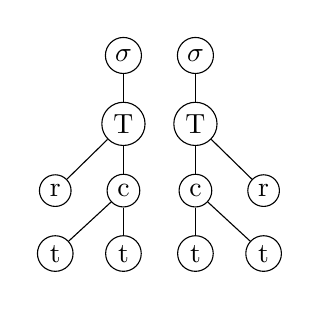
\begin{tikzpicture} [baseline = (y1.base)]
\matrix (m) [matrix of nodes, column sep = 1em, row sep = 1em]{
& \node[draw,circle, inner sep =2pt](x1){$\sigma$};  &  \node[draw,circle, inner sep =2pt](x2){$\sigma$};  \\
& \node[draw,circle, inner sep =2pt](y1){T}; &   \node[draw,circle, inner sep =2pt](y2){T}; \\
\node[draw,circle, inner sep =2pt](z1){r}; & \node[draw,circle, inner sep =2pt](z2){c}; &   \node[draw,circle, inner sep =2pt](z3){c}; & \node[draw,circle, inner sep =2pt](z4){r}; \\
\node[draw,circle, inner sep =2pt](t1){t}; & \node[draw,circle, inner sep =2pt](t2){t}; &  \node[draw,circle, inner sep =2pt](t3){t}; & \node[draw,circle, inner sep =2pt](t4){t}; \\
};
\draw (x1) -- (y1);
\draw (x2) -- (y2);
\draw (z1) -- (y1);
\draw (z2) -- (y1);
\draw (z2) -- (t1);
\draw (z2) -- (t2);
\draw (y2) -- (z3);
\draw (y2) -- (z4);
\draw (z3) -- (t3);
\draw (z3) -- (t4);
\end{tikzpicture}
$\rightarrow$
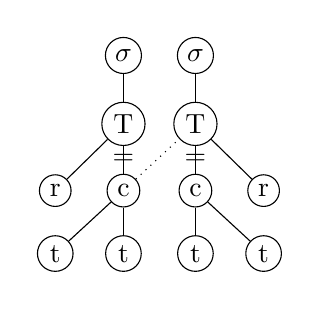
\begin{tikzpicture} [baseline = (y1.base)]
\matrix (m) [matrix of nodes, column sep = 1em, row sep = 1em]{
& \node[draw,circle, inner sep =2pt](x1){$\sigma$};  &  \node[draw,circle, inner sep =2pt](x2){$\sigma$};  \\
& \node[draw,circle, inner sep =2pt](y1){T}; &   \node[draw,circle, inner sep =2pt](y2){T}; \\
\node[draw,circle, inner sep =2pt](z1){r}; & \node[draw,circle, inner sep =2pt](z2){c}; &   \node[draw,circle, inner sep =2pt](z3){c}; & \node[draw,circle, inner sep =2pt](z4){r}; \\
\node[draw,circle, inner sep =2pt](t1){t}; & \node[draw,circle, inner sep =2pt](t2){t}; &  \node[draw,circle, inner sep =2pt](t3){t}; & \node[draw,circle, inner sep =2pt](t4){t}; \\
};
\draw (x1) -- (y1);
\draw (x2) -- (y2);
\draw (z1) -- (y1);
\path (z2) edge node{=} (y1);
\draw (z2) -- (t1);
\draw (z2) -- (t2);
\path (z3) edge node{=} (y2);
\draw (y2) -- (z4);
\draw (z3) -- (t3);
\draw (z3) -- (t4);
\draw [dotted] (z2) -- (y2);
\end{tikzpicture}
$\rightarrow$
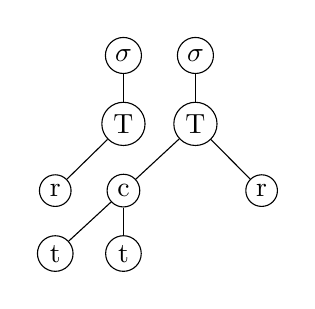
\begin{tikzpicture} [baseline = (y1.base)]
\matrix (m) [matrix of nodes, column sep = 1em, row sep = 1em]{
& \node[draw,circle, inner sep =2pt](x1){$\sigma$};  &  \node[draw,circle, inner sep =2pt](x2){$\sigma$};  \\
& \node[draw,circle, inner sep =2pt](y1){T}; &   \node[draw,circle, inner sep =2pt](y2){T}; \\
\node[draw,circle, inner sep =2pt](z1){r}; & \node[draw,circle, inner sep =2pt](z2){c}; & & \node[draw,circle, inner sep =2pt](z4){r}; \\
\node[draw,circle, inner sep =2pt](t1){t}; & \node[draw,circle, inner sep =2pt](t2){t};  \\
};
\draw (x1) -- (y1);
\draw (x2) -- (y2);
\draw (z1) -- (y1);
\draw (z2) -- (t1);
\draw (z2) -- (t2);
\draw (y2) -- (z4);
\draw (z2) -- (y2);
\end{tikzpicture}
\end{center}
In the figure above, three important structural changes to the input comprise the `contour-shift'. First, the contour node on the first syllable (which dominates the first two terminal tonal nodes) delinks from the tonal root. Next, it forms a new relation with the root `T' node on the second syllable (the `shift'). Finally, the contour node on the second syllable delinks from the root node `T' on the second syllable. We assume that contour (and therefore terminal tonal) nodes that are not linked to a root node are deleted from the structure. Additionally, the result of this process is that the root `T' node in the first syllable does not dominate a `c' node (we will consider the `default l rule' which rectifies this later). Let $\tau^{B}_{zh}$, then, be a transduction which models this process on the input form /LM.HM/ in Bao's representation ($\mathcal{M}^{B}_{I}$):
\begin{equation}
\begin{aligned}
P^1_{\sigma}(x)&\myeq P_{\sigma}(x) & P^1_{T}(x)&\myeq P_{T}(x) \\
P^1_{+u}(x)&\myeq P_{+u}(x) & P^1_{-u}(x)&\myeq P_{-u}(x) \\
P^1_{c}(x)&\myeq P_{c}(x)\land pnlt(x) & P^1_{h}(x)&\myeq P_{h}(x)\land \delta(pnlt(x)) \\
P^1_{l}(x)&\myeq P_{l}(x)\land \delta(pnlt(x)) & \alpha^{1,1}(x)\ap y&\myeq \alpha(x)\ap y \\
\delta^{1,1}(x)\ap y &\myeq \big(P_{r}(x)\land P_{T}(y)\land \delta(x)\ap y\big) \lor & succ^{1,1}(x)\ap y &\myeq succ(x)\ap y \\
&\quad \big(P_{c}(x)\land P_{T}(y)\land pnlt(x) \land last(y)\big)\lor \\
&\quad \big(P_{t}(x)\land P_{c}(y)\land \delta(pnlt(x))\land pnlt(y)\big) \\
\end{aligned}
\end{equation}
Applied to $\mathcal{M}^{B}_{I}$, the resulting model ($\mathcal{M}^{B}_{O}$) is as below:
\begin{center}
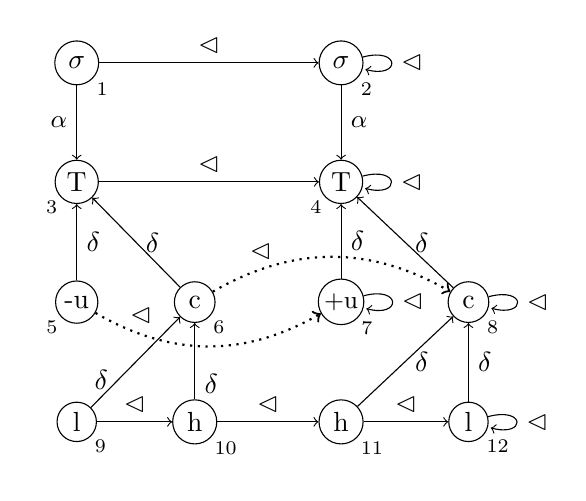
\begin{tikzpicture} [baseline = (y.base)]
\matrix (m) [matrix of nodes, column sep = 2em, row sep = 2em]{
\node[draw,circle, inner sep =3pt, label ={[label distance = -3pt] below right:\scriptsize1}](x){$\sigma$}; & &  \node[draw,circle, inner sep =3pt, label ={[label distance = -3pt] below right:\scriptsize2}](x2){$\sigma$};\\
\node[draw,circle, inner sep =2pt, label ={[label distance = -3pt] below left:\scriptsize3}](y){T}; & & \node[draw,circle, inner sep =2pt, label ={[label distance = -3pt] below left:\scriptsize4}](y2){T};& \\
\node[draw,circle, inner sep =2pt, label ={[label distance = -3pt] below left:\scriptsize5}](z){-u};  & \node[draw,circle, inner sep =3pt, label ={[label distance = -3pt] below right:\scriptsize6}](z1){c}; & \node[draw,circle, inner sep =1pt, label ={[label distance = -3pt] below right:\scriptsize7}](z2){\se u}; & \node[draw,circle, inner sep =3pt, label ={[label distance = -3pt] below right:\scriptsize8}](z3){c}; \\
\node[draw,circle, inner sep =2.5pt, label ={[label distance = -3pt] below right:\scriptsize9}](t){l};& \node[draw,circle, inner sep =2.5pt, label ={[label distance = -3pt] below right:\scriptsize10}](t1){h}; & \node[draw,circle, inner sep =2.5pt, label ={[label distance = -3pt] below right:\scriptsize11}](t2){h}; & \node[draw,circle, inner sep =2.5pt, label ={[label distance = -3pt] below right:\scriptsize12}](t3){l}; \\
};
\draw [->](x) -- (y) node[left, pos=.5]{\small$\alpha$};
\draw [->](z) -- (y) node[right, pos=.5]{$\delta$};
\draw [->](z1) -- (y) node[right, pos=.5]{$\delta$};
\draw [->](x2) -- (y2) node[right, pos=.5]{\small$\alpha$};
\draw [->](z2) -- (y2) node[right, pos=.5]{$\delta$};
\draw [->](t1) -- (z1) node[right, pos=.2]{$\delta$};
\draw [->](t) -- (z1) node[left, pos=.3]{$\delta$};
\draw [->](t2) -- (z3) node[right, pos=.5]{$\delta$};
\draw [->](t3) -- (z3) node[right, pos=.5]{$\delta$};
\draw [->](z3) -- (y2) node[right, pos=.5]{$\delta$};
\draw [->](x) -- (x2) node[above, pos=.5]{$\vartriangleleft$};
\draw [->](t) -- (t1) node[above, pos=.5]{$\vartriangleleft$};
\draw [->](t1) -- (t2) node[above, pos=.5]{$\vartriangleleft$};
\draw [->](t2) -- (t3) node[above, pos=.5]{$\vartriangleleft$};
\draw [->](y) -- (y2) node[above, pos=.5]{$\vartriangleleft$};
\path (x2) edge [loop right] node{$\vartriangleleft$} (x2);
\path (y2) edge [loop right] node{$\vartriangleleft$} (y2);
\path (z3) edge [loop right] node{$\vartriangleleft$} (z3);
\path (z2) edge [loop right] node{$\vartriangleleft$} (z2);
\path (t3) edge [loop right] node{$\vartriangleleft$} (t3);
\path [thick, dotted, ->] (z) edge [bend right=30] node[above,pos=.2]{$\vartriangleleft$} (z2);
\path [thick, dotted, ->] (z1) edge [bend left=30] node[above,pos=.2]{$\vartriangleleft$} (z3);
\end{tikzpicture}
\hspace{1cm}
$\mapsto$
\hspace{1cm}
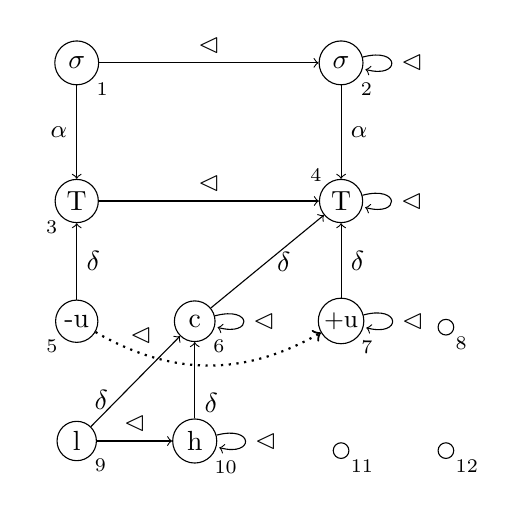
\begin{tikzpicture} [baseline = (y.base)]
\matrix (m) [matrix of nodes, column sep = 2em, row sep = 2em]{
\node[draw,circle, inner sep =3pt, label ={[label distance = -3pt] below right:\scriptsize1}](x){$\sigma$}; & &  \node[draw,circle, inner sep =3pt, label ={[label distance = -3pt] below right:\scriptsize2}](x2){$\sigma$};\\
\node[draw,circle, inner sep =2pt, label ={[label distance = -3pt] below left:\scriptsize3}](y){T}; & & \node[draw,circle, inner sep =2pt, label ={[label distance = -3pt] above left:\scriptsize4}](y2){T};& \\
\node[draw,circle, inner sep =2pt, label ={[label distance = -3pt] below left:\scriptsize5}](z){-u};  & \node[draw,circle, inner sep =3pt, label ={[label distance = -3pt] below right:\scriptsize6}](z1){c}; & \node[draw,circle, inner sep =1pt, label ={[label distance = -3pt] below right:\scriptsize7}](z2){\se u}; & \node[draw,circle, inner sep =2pt, label ={[label distance = -3pt] below right:\scriptsize8}](z3){\hspace{1em}}; \\
\node[draw,circle, inner sep =2.5pt, label ={[label distance = -3pt] below right:\scriptsize9}](t){l};& \node[draw,circle, inner sep =2.5pt, label ={[label distance = -3pt] below right:\scriptsize10}](t1){h}; & \node[draw,circle, inner sep =2pt, label ={[label distance = -3pt] below right:\scriptsize11}](t2){\hspace{1em}}; & \node[draw,circle, inner sep =2pt, label ={[label distance = -3pt] below right:\scriptsize12}](t3){\hspace{1em}}; \\
};
\draw [->](x) -- (y) node[left, pos=.5]{\small$\alpha$};
\draw [->](z) -- (y) node[right, pos=.5]{$\delta$};
\draw [->](z1) -- (y2) node[right, pos=.5]{$\delta$};
\draw [->](x2) -- (y2) node[right, pos=.5]{\small$\alpha$};
\draw [->](z2) -- (y2) node[right, pos=.5]{$\delta$};
\draw [->](t1) -- (z1) node[right, pos=.2]{$\delta$};
\draw [->](t) -- (z1) node[left, pos=.3]{$\delta$};
\draw [->](x) -- (x2) node[above, pos=.5]{$\vartriangleleft$};
\draw [->](t) -- (t1) node[above, pos=.5]{$\vartriangleleft$};
\draw [->](y) -- (y2) node[above, pos=.5]{$\vartriangleleft$};
\path (x2) edge [loop right] node{$\vartriangleleft$} (x2);
\path (y2) edge [loop right] node{$\vartriangleleft$} (y2);
\path (z2) edge [loop right] node{$\vartriangleleft$} (z2);
\path (z1) edge [loop right] node{$\vartriangleleft$} (z1);
\path (t1) edge [loop right] node{$\vartriangleleft$} (t1);
\path [thick, dotted, ->] (z) edge [bend right=30] node[above,pos=.2]{$\vartriangleleft$} (z2);
\end{tikzpicture}
\end{center}
We can also define the output model explicitly:
\begin{equation} \label{Mbo}
\begin{aligned}
\mathcal{M}^{B}_{O} \myeq \langle \mathcal{D}; &P_{\sigma}, P_{T}, P_{+u}, P_{-u}, P_{h}, P_{l}, P_{c}; \\
\alpha(x)\ap y, &\delta(x)\ap y, succ(x)\ap y \rangle \\
\mathcal{D} &= \{1, 2, 3, 4, 5, 6, 7, 8, 9, 10, 11, 12\}  \\
P_{\sigma} &= \{1, 2\} & P_{T} &= \{3, 4\} \\
P_{+u} &= \{7\} & P_{-u} &= \{5\} \\
P_{h} &= \{10\} & P_{l} &= \{9\} \\ 
P_{c} &= \{6\}& \alpha(x)\ap y &= \begin{cases} 3 & x=1 \\ 4 & x=2 \end{cases}  \\
 \delta(x)\ap y &= \begin{cases} 3 & x=5 \\ 4 & x\in \{6,7\} \\ 6 & x\in\{9,10\} \\ \end{cases} &
succ(x)\ap y &= \begin{cases} 2 & x\in \{1,2\} \\ 4 & x\in \{3,4\} \\ 7 & x\in\{5,7\} \\ 6 & x=6,8 \\ 10 & x\in\{9,10\} \end{cases} \\
\end{aligned}
\end{equation}
In this transduction, unary predicates over syllable and register nodes are preserved from the input structure. Unary relations which label `c' and terminal tonal nodes are defined such that they preserve only the `c' and `t' nodes from the penultimate (in this case, first) syllable. This, in effect, `deletes' the contour information from the second syllable. Association between TBUs and tonal roots is identical between input and output forms. Defining the dominance function $\delta(x)\ap y$ aims to maintain the relations between register and `T' nodes (first conjunct) and (penultimate) `c' and `t' nodes (third conjunct), but defines `T' to 'c' dominance as a relation that holds between the \emph{penultimate} `c' and the \emph{final} `T' (second conjunct), effectively shifting the contour node one syllable to the right. The ordering relations are preserved between input and output.\footnote{This isn't necessarily true. In particular, the surviving `c' node is no longer succeeded by another `c' node; it is the final node on its tier in the output. The same is true for the `h' terminal node dominated by that `c' node. We can offer an explicit definition of successor on the output model such that all fully-preserved tiers have the same ordering. So, for some tier element $\epsilon$: $succ(x)\ap y \myeq P_{\epsilon}(x)\land P_{\epsilon}(y)\land succ(x)\ap y$. This definition will apply to syllable, `T', and register nodes. To account for the fact that penultimate `c' is now final (its own successor) and for the new situation with the terminal nodes, we add several disjuncts to that definition and join them by disjunction: \\
$succ^{1,1}(x)\ap y\myeq (P_{c}(x)\land P_{c}(y)\land pnlt(x)\land pnlt(y)\land x\ap y) \lor \\
(P_{l}(x)\land P_{h}(y)\land \delta(succ(x))\land\delta(succ(y))\land succ(x)\ap y) \lor \\
(P_{h}(x)\land P_{h}(y)\land \delta(succ(x))\land\delta(succ(y))\land x\ap y)$}
\subsection{General Transduction on Bao Output: $\Gamma^{by}: \mathcal{M}^{B}_{O} \mapsto \mathcal{M}^{Y}_{O}$}
Now, we perform the transduction $\Gamma^{by}$ on the model in (\ref{Mbo})---that is, the output of $\tau^{B}_{zh}$---to yield a model of a contour-shifted structure in Yip's representation.
\begin{center}
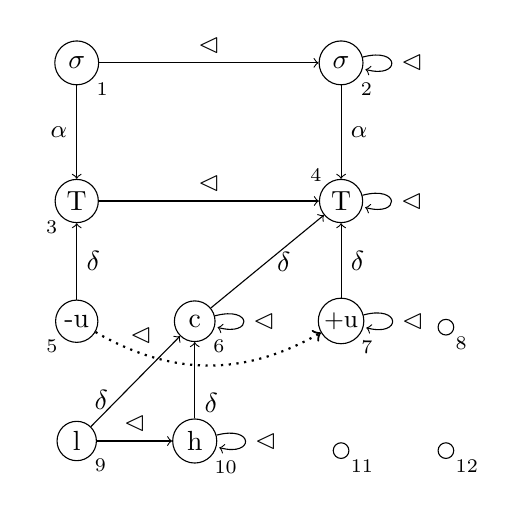
\begin{tikzpicture} [baseline = (y.base)]
\matrix (m) [matrix of nodes, column sep = 2em, row sep = 2em]{
\node[draw,circle, inner sep =3pt, label ={[label distance = -3pt] below right:\scriptsize1}](x){$\sigma$}; & &  \node[draw,circle, inner sep =3pt, label ={[label distance = -3pt] below right:\scriptsize2}](x2){$\sigma$};\\
\node[draw,circle, inner sep =2pt, label ={[label distance = -3pt] below left:\scriptsize3}](y){T}; & & \node[draw,circle, inner sep =2pt, label ={[label distance = -3pt] above left:\scriptsize4}](y2){T};& \\
\node[draw,circle, inner sep =2pt, label ={[label distance = -3pt] below left:\scriptsize5}](z){-u};  & \node[draw,circle, inner sep =3pt, label ={[label distance = -3pt] below right:\scriptsize6}](z1){c}; & \node[draw,circle, inner sep =1pt, label ={[label distance = -3pt] below right:\scriptsize7}](z2){\se u}; & \node[draw,circle, inner sep =2pt, label ={[label distance = -3pt] below right:\scriptsize8}](z3){\hspace{1em}}; \\
\node[draw,circle, inner sep =2.5pt, label ={[label distance = -3pt] below right:\scriptsize9}](t){l};& \node[draw,circle, inner sep =2.5pt, label ={[label distance = -3pt] below right:\scriptsize10}](t1){h}; & \node[draw,circle, inner sep =2pt, label ={[label distance = -3pt] below right:\scriptsize11}](t2){\hspace{1em}}; & \node[draw,circle, inner sep =2pt, label ={[label distance = -3pt] below right:\scriptsize12}](t3){\hspace{1em}}; \\
};
\draw [->](x) -- (y) node[left, pos=.5]{\small$\alpha$};
\draw [->](z) -- (y) node[right, pos=.5]{$\delta$};
\draw [->](z1) -- (y2) node[right, pos=.5]{$\delta$};
\draw [->](x2) -- (y2) node[right, pos=.5]{\small$\alpha$};
\draw [->](z2) -- (y2) node[right, pos=.5]{$\delta$};
\draw [->](t1) -- (z1) node[right, pos=.2]{$\delta$};
\draw [->](t) -- (z1) node[left, pos=.3]{$\delta$};
\draw [->](x) -- (x2) node[above, pos=.5]{$\vartriangleleft$};
\draw [->](t) -- (t1) node[above, pos=.5]{$\vartriangleleft$};
\draw [->](y) -- (y2) node[above, pos=.5]{$\vartriangleleft$};
\path (x2) edge [loop right] node{$\vartriangleleft$} (x2);
\path (y2) edge [loop right] node{$\vartriangleleft$} (y2);
\path (z2) edge [loop right] node{$\vartriangleleft$} (z2);
\path (z1) edge [loop right] node{$\vartriangleleft$} (z1);
\path (t1) edge [loop right] node{$\vartriangleleft$} (t1);
\path [thick, dotted, ->] (z) edge [bend right=30] node[above,pos=.2]{$\vartriangleleft$} (z2);
\end{tikzpicture}
\hspace{1cm}
$\mapsto$
\hspace{1cm}
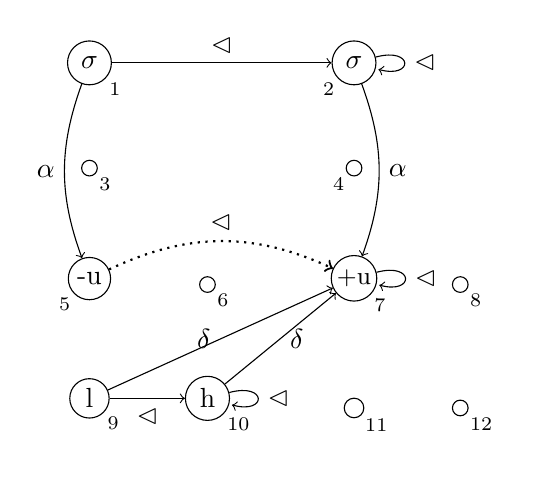
\begin{tikzpicture} [baseline = (y.base)]
\matrix (m) [matrix of nodes, column sep = 2em, row sep = 2em]{
\node[draw,circle, inner sep =3pt, label ={[label distance = -3pt] below right:\scriptsize1}](x){$\sigma$}; & &  \node[draw,circle, inner sep =3pt, label ={[label distance = -3pt] below left:\scriptsize2}](x2){$\sigma$};\\
\node[draw,circle, inner sep =2pt, label ={[label distance = -3pt] below right:\scriptsize3}](y){\hspace{1em}}; & & \node[draw,circle, inner sep =2pt, label ={[label distance = -3pt] below left:\scriptsize4}](y2){\hspace{1em}};& \\
\node[draw,circle, inner sep =2pt, label ={[label distance = -3pt] below left:\scriptsize5}](z){-u};  & \node[draw,circle, inner sep =2pt, label ={[label distance = -3pt] below right:\scriptsize6}](z1){\hspace{1em}}; & \node[draw,circle, inner sep =1pt, label ={[label distance = -3pt] below right:\scriptsize7}](z2){\se u}; & \node[draw,circle, inner sep =2pt, label ={[label distance = -3pt] below right:\scriptsize8}](z3){\hspace{1em}}; \\
\node[draw,circle, inner sep =2.5pt, label ={[label distance = -3pt] below right:\scriptsize9}](t){l};& \node[draw,circle, inner sep =2.5pt, label ={[label distance = -3pt] below right:\scriptsize10}](t1){h}; & \node[draw,circle, inner sep =2.5pt, label ={[label distance = -3pt] below right:\scriptsize11}](t2){\hspace{1em}}; & \node[draw,circle, inner sep =2pt, label ={[label distance = -3pt] below right:\scriptsize12}](t3){\hspace{1em}}; \\
};
\draw [->](x) -- (x2) node[above, pos=.5]{$\vartriangleleft$};
\draw [->](t) -- (t1) node[below, pos=.5]{$\vartriangleleft$};
\draw [->](t) -- (z2) node[left, pos=.5]{$\delta$};
\draw [->](t1) -- (z2) node[right, pos=.5]{$\delta$};
\path (x2) edge [loop right] node{$\vartriangleleft$} (x2);
\path (z2) edge [loop right] node{$\vartriangleleft$} (z2);
\path (t1) edge [loop right] node{$\vartriangleleft$} (t1);
\path [thick, dotted, ->] (z) edge [bend left=25] node[above]{$\vartriangleleft$} (z2);
\path [->] (x) edge [bend right=20] node[left]{$\alpha$} (z);
\path [->] (x2) edge [bend left=20] node[right]{$\alpha$} (z2);
\end{tikzpicture}
\end{center}
Following the general transduction from a Bao model to a Yip model, the result here is a Yip analog of the result of contour-shift pattern in Bao's representation; as before, the `T', `c', and register nodes fuse into a single node (register), but the output form in terms of its tonal realization [L.MH] is identical across both models.
\subsection{Discussion: Yip to Yip?}
We have performed a series of transductions to explore equivalencies between Yip and Bao models. We applied a QF transduction on a model of Bao's representation to produce a corresponding model in Yip's tonal geometry. We further applied a language-specific QF transduction on that model of Bao's representation to formalize an attested tone sandhi process. The general transduction was applied on the output of the I/O transduction, resulting in a post-contour-shift model in Yip's representation. All transductions were of a simple logical complexity (Quantifier-Free). What we have now is a pair of Yip models, one for a Zhenhai input, and one for a Zhenhai output.
\begin{center}
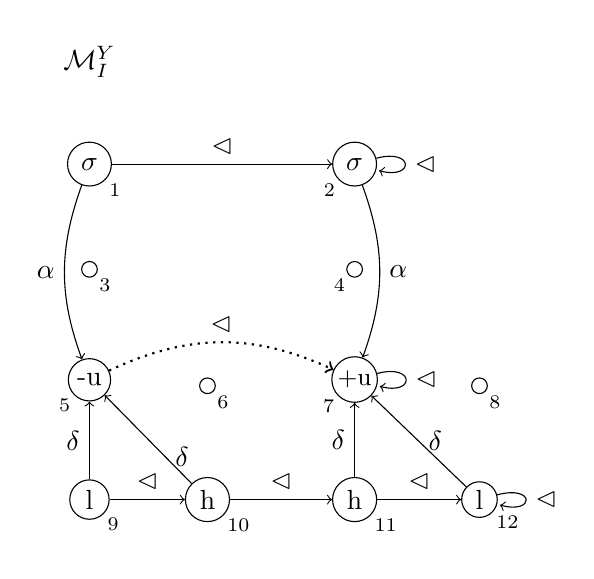
\begin{tikzpicture} [baseline = (y.base)]
\matrix (m) [matrix of nodes, column sep = 2em, row sep = 2em]{
$\mathcal{M}^{Y}_{I}$ \\
\node[draw,circle, inner sep =3pt, label ={[label distance = -3pt] below right:\scriptsize1}](x){$\sigma$}; & &  \node[draw,circle, inner sep =3pt, label ={[label distance = -3pt] below left:\scriptsize2}](x2){$\sigma$};\\
\node[draw,circle, inner sep =2pt, label ={[label distance = -3pt] below right:\scriptsize3}](y){\hspace{1em}}; & & \node[draw,circle, inner sep =2pt, label ={[label distance = -3pt] below left:\scriptsize4}](y2){\hspace{1em}};& \\
\node[draw,circle, inner sep =2pt, label ={[label distance = -3pt] below left:\scriptsize5}](z){-u};  & \node[draw,circle, inner sep =2pt, label ={[label distance = -3pt] below right:\scriptsize6}](z1){\hspace{1em}}; & \node[draw,circle, inner sep =1pt, label ={[label distance = -3pt] below left:\scriptsize7}](z2){\se u}; & \node[draw,circle, inner sep =2pt, label ={[label distance = -3pt] below right:\scriptsize8}](z3){\hspace{1em}}; \\
\node[draw,circle, inner sep =2.5pt, label ={[label distance = -3pt] below right:\scriptsize9}](t){l};& \node[draw,circle, inner sep =2.5pt, label ={[label distance = -3pt] below right:\scriptsize10}](t1){h}; & \node[draw,circle, inner sep =2.5pt, label ={[label distance = -3pt] below right:\scriptsize11}](t2){h}; & \node[draw,circle, inner sep =2pt, label ={[label distance = -3pt] below right:\scriptsize12}](t3){l}; \\
};
\draw [->](x) -- (x2) node[above, pos=.5]{$\vartriangleleft$};
\draw [->](t) -- (t1) node[above, pos=.5]{$\vartriangleleft$};
\draw [->](t1) -- (t2) node[above, pos=.5]{$\vartriangleleft$};
\draw [->](t2) -- (t3) node[above, pos=.5]{$\vartriangleleft$};
\draw [->](t) -- (z) node[left, pos=.5]{$\delta$};
\draw [->](t1) -- (z) node[right, pos=.3]{$\delta$};
\draw [->](t2) -- (z2) node[left, pos=.5]{$\delta$};
\draw [->](t3) -- (z2) node[right, pos=.5]{$\delta$};
\path (x2) edge [loop right] node{$\vartriangleleft$} (x2);
\path (z2) edge [loop right] node{$\vartriangleleft$} (z2);
\path (t3) edge [loop right] node{$\vartriangleleft$} (t3);
\path [thick, dotted, ->] (z) edge [bend left=25] node[above]{$\vartriangleleft$} (z2);
\path [->] (x) edge [bend right=20] node[left]{$\alpha$} (z);
\path [->] (x2) edge [bend left=20] node[right]{$\alpha$} (z2);
\end{tikzpicture}
\hspace{2.2cm}
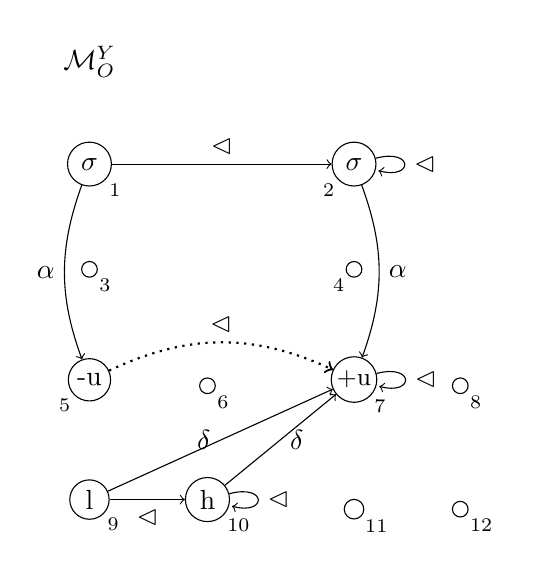
\begin{tikzpicture} [baseline = (y.base)]
\matrix (m) [matrix of nodes, column sep = 2em, row sep = 2em]{
$\mathcal{M}^{Y}_{O}$ \\
\node[draw,circle, inner sep =3pt, label ={[label distance = -3pt] below right:\scriptsize1}](x){$\sigma$}; & &  \node[draw,circle, inner sep =3pt, label ={[label distance = -3pt] below left:\scriptsize2}](x2){$\sigma$};\\
\node[draw,circle, inner sep =2pt, label ={[label distance = -3pt] below right:\scriptsize3}](y){\hspace{1em}}; & & \node[draw,circle, inner sep =2pt, label ={[label distance = -3pt] below left:\scriptsize4}](y2){\hspace{1em}};& \\
\node[draw,circle, inner sep =2pt, label ={[label distance = -3pt] below left:\scriptsize5}](z){-u};  & \node[draw,circle, inner sep =2pt, label ={[label distance = -3pt] below right:\scriptsize6}](z1){\hspace{1em}}; & \node[draw,circle, inner sep =1pt, label ={[label distance = -3pt] below right:\scriptsize7}](z2){\se u}; & \node[draw,circle, inner sep =2pt, label ={[label distance = -3pt] below right:\scriptsize8}](z3){\hspace{1em}}; \\
\node[draw,circle, inner sep =2.5pt, label ={[label distance = -3pt] below right:\scriptsize9}](t){l};& \node[draw,circle, inner sep =2.5pt, label ={[label distance = -3pt] below right:\scriptsize10}](t1){h}; & \node[draw,circle, inner sep =2.5pt, label ={[label distance = -3pt] below right:\scriptsize11}](t2){\hspace{1em}}; & \node[draw,circle, inner sep =2pt, label ={[label distance = -3pt] below right:\scriptsize12}](t3){\hspace{1em}}; \\
};
\draw [->](x) -- (x2) node[above, pos=.5]{$\vartriangleleft$};
\draw [->](t) -- (t1) node[below, pos=.5]{$\vartriangleleft$};
\draw [->](t) -- (z2) node[left, pos=.5]{$\delta$};
\draw [->](t1) -- (z2) node[right, pos=.5]{$\delta$};
\path (x2) edge [loop right] node{$\vartriangleleft$} (x2);
\path (z2) edge [loop right] node{$\vartriangleleft$} (z2);
\path (t1) edge [loop right] node{$\vartriangleleft$} (t1);
\path [thick, dotted, ->] (z) edge [bend left=25] node[above]{$\vartriangleleft$} (z2);
\path [->] (x) edge [bend right=20] node[left]{$\alpha$} (z);
\path [->] (x2) edge [bend left=20] node[right]{$\alpha$} (z2);
\end{tikzpicture}
\end{center}
The question we want to ask is: does there exist some transduction $\tau^{Y}_{zh}$ from $\mathcal{M}^{Y}_{I}$ to $\mathcal{M}^{Y}_{O}$, and, crucially, is it QF? Yes; we define such a transduction below, and base it on the definition of $\tau^{B}_{zh}$:
\begin{equation}
\begin{aligned}
P^1_{\sigma}(x)&\myeq P_{\sigma}(x) & P^1_{+u}(x)&\myeq P_{+u}(x) \\
P^1_{-u}(x)&\myeq P_{-u}(x) & P^1_{h}(x)&\myeq P_{h}(x)\land \delta(pnlt(x)) \\
P^1_{l}(x)&\myeq P_{l}(x)\land \delta(pnlt(x)) & \alpha^{1,1}(x)\ap y&\myeq \alpha(x)\ap y \\
\delta^{1,1}(x)\ap y&\myeq P_{t}(x)\land P_{r}(y)\land & succ^{1,1}(x)\ap y&\myeq \big(P_{\sigma}(x)\land P_{\sigma}(y)\land succ(x)\ap y\big)\lor \\
&\quad \delta(pnlt(x))\land last(y) & &\quad \big(P_{r}(x)\land P_{r}(y)\land succ(x)\ap y \big)\lor \\
& & &\quad \big(P_{l}(x)\land P_{h}(y)\land \delta(pnlt(x))\land\\
& & &\quad \delta(pnlt(y)) \land succ(x)\ap y\big) \lor \\
& & &\quad \big(P_{h}(x)\land P_{h}(y)\land \delta(pnlt(x))\land \\
& & &\quad \delta(pnlt(y))\land x\ap y\big) \\
\end{aligned}
\end{equation}
In this definition, syllable and register nodes are defined as normal. Definitions of terminal node unary predicates are identical across $\tau^{B}_{zh}$ and $\tau^{Y}_{zh}$; that is, they both identify tones that are immediately dominated by a \emph{penult}. In Bao's model, this is the `c' node on the first syllable, while in Yip's model, it is the register node on the first syllable (recall the structural equivalency of these nodes). As association between TBU and register nodes does not change, the binary function $\alpha^{1,1}(x)\ap y$ is defined in terms of input association. \par
The definition of the dominance function is crucial here. It is, in essence, a condensed version of the same definition in $\tau^{B}_{zh}$. Both are compared below:
\begin{equation}
\begin{aligned}
&\tau^{Y}_{zh} & &\tau^{B}_{zh} \\
\delta^{1,1}(x)\ap y&\myeq P_{t}(x)\land P_{r}(y)\land & \delta^{1,1}(x)\ap y &\myeq \big(P_{r}(x)\land P_{T}(y)\land \delta(x)\ap y\big)\lor \\
&\quad \delta(pnlt(x))\land last(y) & &\quad \big(P_{c}(x)\land P_{T}(y)\land pnlt(x)\land last(y)\big)\lor \\
& & &\quad \big(P_{t}(x)\land P_{c}(y)\land \delta(pnlt(x))\land pnlt(y)\big)\\
\end{aligned}
\end{equation}
The last two conjuncts of the $\tau^{Y}_{zh}$ definition are a combination of those of the second and third disjuncts in the $\tau^{B}_{zh}$ definition. Again, this reflects the structural equivalence of `c' nodes in Bao's representation and register nodes in Yip's. \par
To impose the correct order on elements (specifically on the terminal tonal tier), the successor function must be defined such that only `l' and 'h' from the first syllable are in some order, and so that the `h' node from the first syllable is now the final node in that tier (i.e. it is its own successor). What is important to keep in mind here is that this reordering is possible (as is the rest of the transduction) using QF logic. \par
Intuitively, this result should follow directly from the equivalency between the models that we proved in the preceding sections. If the models are equivalent, then processes that map one structure to another in the same model should also be equivalent within a certain scope of logical complexity. We have shown that Yip and Bao tonal geometries are QF bi-interpretable. Any process that can be formalized in Bao's representation can also be formalized in Yip's representation.
\end{document}